\documentclass[11pt,a4paper]{scrartcl}

% ---- Paquetes ----
\usepackage[utf8]{inputenc}
\usepackage[T1]{fontenc}
\usepackage[spanish]{babel}
\usepackage{graphicx}
\usepackage{amsmath}
\usepackage{xcolor}
\usepackage{caption}
\usepackage{subcaption}
\usepackage{float}
\usepackage{booktabs}
\usepackage{longtable}
\usepackage{tikz}
\usetikzlibrary{positioning,arrows.meta,angles,quotes,calc}
\usepackage[margin=2.2cm]{geometry}
\usepackage[colorlinks=true,linkcolor=black,citecolor=black,urlcolor=blue]{hyperref}
% biblatex+biber cambiado a bibtex clasico (30-ago-2026): el .bib solo usa
% campos estandar de BibTeX (sin fechas ISO, sin location, sin urldate) y el
% documento solo usa \cite{} plano (sin \parencite/\textcite) - biber es el
% paso mas pesado de compilar (proceso externo aparte, con su propio
% arranque) y biblatex el paquete mas lento de cargar de todo el preambulo;
% con 10 entradas nomas, bibtex hace exactamente lo mismo mucho mas rapido -
% pensado para bajar el tiempo de compilacion en el plan gratuito de Overleaf.
\usepackage{listings}

% Etiquetas de trazabilidad: literatura / aporte propio / implementación MATLAB / pendiente de tu revisión
\newcommand{\fuente}[1]{\par\noindent{\color{blue!55!black}\small\textbf{Fuente:} #1}\par}
\newcommand{\aporte}[1]{\par\noindent{\color{orange!75!black}\small\textbf{Aporte propio:} #1}\par}
\newcommand{\matlabtitle}[1]{\par\noindent{\color{green!35!black}\small\textbf{MATLAB --- código real:} #1}\vspace{-2pt}}
\newcommand{\revisar}[1]{\par\noindent{\color{red!55!black}\small\textbf{Pendiente de tu revisión:} #1}\par}
\newcommand{\resuelto}[1]{\par\noindent{\color{green!35!black}\small\textbf{Resuelto:} #1}\par}
% Recuadro Entra/Sale de cada Paso del pipeline: qué variable toma de qué
% paso anterior, y qué produce para el siguiente --- pedido explícito del
% usuario, para que la cadena de dependencia entre pasos sea escaneable de
% un vistazo, no una oración densa de leer.
\newcommand{\entradasalida}[2]{%
\par\noindent\fcolorbox{violet!40!black}{violet!4}{%
\begin{minipage}{0.965\linewidth}\small
\textbf{\textcolor{violet!55!black}{$\rightarrow$ Entra:}} #1\\[3pt]
\textbf{\textcolor{violet!55!black}{$\leftarrow$ Sale:}} #2
\end{minipage}}\par\vspace{4pt}}

\lstset{
  language=Matlab,
  basicstyle=\ttfamily\scriptsize,
  keywordstyle=\color{blue!55!black},
  commentstyle=\color{gray!70!black}\itshape,
  numbers=none,
  breaklines=true,
  frame=single,
  rulecolor=\color{green!35!black},
  backgroundcolor=\color{green!4},
  xleftmargin=0.4cm,
  aboveskip=2pt,
  belowskip=6pt,
  showstringspaces=false
}

\title{Generación de trayectorias de rodilla, tobillo e inclinación tibial a partir de antropometría: selección y validación de modelo mediante datos independientes}
\subtitle{Informe técnico de proceso --- versión para asesores}
\author{Luis Marcos Plasencia Janampa \\ \small Laboratorio LIBRA, Pontificia Universidad Católica del Perú \\ \small \href{mailto:luis.plasencia@pucp.edu.pe}{luis.plasencia@pucp.edu.pe}}
\date{\today}

\begin{document}
\shorthandoff{<>}

\maketitle
\tableofcontents
\newpage

\noindent\textbf{Cómo leer este informe.} Cuatro etiquetas de color marcan el origen de cada afirmación:
\fuente{de dónde viene (fuente publicada, con la parte exacta citada).}
\aporte{qué decidimos/calculamos/combinamos nosotros, no reportado así en ninguna fuente individual.}

\matlabtitle{el código real (copiado del proyecto, no reescrito ni resumido en prosa) para los pasos donde la literatura no da algo listo para usar tal cual --- para que el asesor vea exactamente qué se ejecutó, sin tener que abrir MATLAB. Esto es solo para nosotros: al artículo de revista no va ningún código.}

\revisar{cualquier coeficiente, signo o celda que no pudimos verificar con total certeza contra la fuente original --- se marca así en vez de darlo por resuelto en silencio, para que alguien lo revise antes de que el informe se dé por definitivo.}

\bigskip

\section{Resumen}

\begin{itemize}
    \item El generador convierte talla, masa y sexo en la trayectoria de referencia del simulador de 3 GDL (LIBRA-PUCP), sin depender de una captura pregrabada de un sujeto.
    \item Se probaron 3 modelos publicados (Koopman 2014, Zhao 2026, Yun 2014), sin reentrenar, contra 5 bases de datos independientes (1 a 246 sujetos).
    \item \textbf{Koopman 2014 ganó en los tres segmentos} (rodilla, tobillo, ángulo tibial). El ángulo tibial tiene su propia calibración (LOSO) que corrige una sobreestimación de 20--23\,\% en amplitud angular. Para la posición final de rodilla/tobillo (péndulo doble + cadera oscilatoria, Sección~\ref{sec:paso4}) se corrige la posición ya generada (Sección~\ref{sec:retrocesos_x}), un método distinto por eje: deformación de tiempo (\emph{warp}) en $X$, serie de Fourier en $Y$.
    \item \textbf{Resultado final, con la ÚNICA entrada que la app realmente pide (talla --- masa/muslo/tibia/velocidad se estiman, nunca se miden):} rodilla y tobillo quedan en RMSEnorm 0.89--1.17 ($r$=0.949--0.999, $N$=44), ángulo tibial en RMSEnorm 1.01 ($r$=0.989, $N$=47) --- Excelente/Bueno en las 5 curvas (Tabla~\ref{tab:resultados_finales}). Además, el avance ($X$) queda \textbf{garantizado monótono en talla} (a mayor talla, igual o mayor avance, siempre --- Sección~\ref{sec:retrocesos_x}), una propiedad matemática del método, no un ajuste casual. Es más pobre que una primera versión de esta validación que sí usaba antropometría/velocidad reales de \emph{Kuopio} (RMSEnorm 0.52--0.92) --- ese primer número no representaba lo que un usuario real de la app obtiene, así que se reajustó por completo (\texttt{Refit\_CorreccionFinal\_TallaSola.m}, 31-ago-2026, y \texttt{Ajustar\_Warp\_Temporal\_TallaSola.m}, 01-sep-2026) y se reemplazó en este informe.
    \item Hallazgo propio adicional: Zhao y Yun tienen un defecto de fase de 50\,\% del ciclo en su parámetro de lateralidad --- explica por qué parecían competitivos en algunas bases y no en otras.
    \item Camargo et al.\ queda reservada, sin usar, como examen final de no-circularidad --- pendiente de ejecutar.
\end{itemize}

La Tabla~\ref{tab:aportes} resume, en una sola vista, qué de este trabajo es literatura aplicada tal cual y qué es aporte propio del proyecto.

\begin{table}[H]
\centering
\caption{Resumen de aportes propios del proyecto, en orden de aparición en este informe.}
\label{tab:aportes}
\small
\begin{tabular}{@{}p{4.6cm}p{1.6cm}p{7.4cm}@{}}
\toprule
Aporte propio & Sección & Por qué no es solo "aplicar la literatura" \\
\midrule
Elegir vía rodilla vs.\ vía tobillo para el ángulo tibial & \ref{sec:reduccion_tibial} & Ninguna fuente lo decide; se probó contra dato real propio ($r=0.982$ vs.\ $-0.435$) \\
Pipeline de 5 pasos que encadena 4 fuentes distintas & \ref{sec:pipeline} & Ninguna fuente individual define este ensamblaje completo \\
Reutilizar la Ec.\ 3 de Koopman como reloj compartido por los 3 candidatos & \ref{sec:paso2} & Koopman no la propone para Zhao/Yun; decisión de ingeniería propia \\
Cadena cinemática de péndulo doble (cadera--rodilla--tobillo, una sola fórmula para todo el ciclo) + cadera oscilatoria verificada contra literatura & \ref{sec:paso4} & Construcción propia; reemplaza un primer modelo con conmutación de fase y artefactos no físicos \\
Exportación en el formato exacto que el simulador ya lee & \ref{sec:paso5} & Ingeniería de integración, no un dato de literatura \\
Calibración afín LOSO del ángulo (corrige sobreestimación de 20--23\,\%) & \ref{sec:calibracion} & Koopman et al.\ no reporta este defecto ni esta corrección \\
Corrección de posición por deformación de tiempo (warp) en $X$, con ecuación diferencial que garantiza monotonía en tiempo Y en talla & \ref{sec:retrocesos_x} & Construcción propia; ninguna fuente combina warp temporal con un afín restringido para garantizar orden físico, ni aplica un método distinto por eje según su naturaleza \\
Hallazgo: desfase de fase de 50\,\% en Zhao/Yun & \ref{sec:comparacion_candidatos} & Encontrado y verificado numéricamente en este proyecto \\
\bottomrule
\end{tabular}
\end{table}

\section{Contexto y objetivo}
\label{sec:contexto}

\begin{itemize}
    \item El simulador de 3 GDL de LIBRA ensaya prótesis transtibiales ejecutando una trayectoria leída de un CSV.
    \item Plan inicial (abandonado 19-ago-2026): reproducir con fidelidad la captura de un único sujeto. Dos problemas: (a) un sujeto no representa la variabilidad poblacional; (b) la fidelidad de seguimiento dependía de una integración Raspberry Pi--ESP32 aún incompleta, que bloqueaba casi toda validación.
    \item Plan vigente: un \textbf{generador} produce la trayectoria desde antropometría, con un modelo tomado de la literatura (no desarrollado por el equipo), validado contra bases públicas ajenas a su construcción.
\end{itemize}

Dos condiciones sostienen la validez del enfoque:
\begin{enumerate}
    \item el modelo debe venir de una fuente publicada, coeficientes verificables, sin reentrenar con datos propios;
    \item la validación debe ser independiente --- ninguna base sirve a la vez para \emph{elegir} el modelo y para \emph{reportar} qué tan bien funciona.
\end{enumerate}

\section{El modelo seleccionado: Koopman et al.\ (2014)}
\label{sec:koopman}

\fuente{Koopman, van Asseldonk \& van der Kooij, \emph{Journal of Biomechanics} 47:1447--1458 (2014).}

\begin{itemize}
    \item Cada uno de 4 ángulos (cadera ab/aducción, cadera flexo-extensión, rodilla flexo-extensión, tobillo plantar/dorsiflexión) es un \emph{spline quíntico de Hermite} por tramos, que empalma en 6 eventos clave del ciclo (0--100\,\%), más un 7\textsuperscript{mo} punto de cierre igual al 1\textsuperscript{ro}, para periodicidad exacta.
    \item En cada evento $i$: posición $x_i$ (\%), ángulo $y_i$ (°), velocidad $\dot y_i$, aceleración $\ddot y_i$. Cada uno se predice con una regresión ya publicada, en función de solo velocidad $v$ (km/h) y talla $l$ (m):
\end{itemize}

\begin{equation}
p(v,l) = \beta_0 + \beta_1 v + \beta_2 v^2 + \beta_3 l
\label{eq:koopman_regresion}
\end{equation}

\fuente{$(\beta_0,\beta_1,\beta_2,\beta_3)$ de las Tablas 1--5 del artículo (24 filas de coeficientes).} Algunos parámetros están fijados por definición del evento (no estimados): $x_1=1\,\text{\%}$; velocidad cero en extremos de posición; aceleración cero en extremos de velocidad.

Las Tablas 1--5 se usaron tal cual, sin adaptar (la literatura ya da la forma lista para calcular: coeficientes $\to$ regresión $\to$ ángulo). Único problema real de conversión: el extractor de texto estándar del PDF perdía los signos negativos de la tabla --- se resolvió re-extrayendo los coeficientes con \texttt{pdfplumber} (Python) antes de pasarlos a MATLAB.

\matlabtitle{coeficientes de \emph{ángulo} ($y_i$) de la Tabla 3 (rodilla) tal como quedaron en el código --- esto es lo mismo que ves impreso en la Tabla~\ref{tab:koopman_rodilla} más abajo, columnas $[\beta_0\ \beta_1(v)\ \beta_2(v^2)\ \beta_3(l)]$ por evento:}
\begin{lstlisting}
T3.coef_y = [31.595   -4.311  0.494 -13.050;   % Contacto de talon
              5.995    3.028  0      0;        % Apoyo maximo
            -10.037    0      0      7.594;    % Apoyo minimo
             29.618    3.803 -0.486  0;        % Max. pend. balanceo
             38.110    9.744 -1.105  0;        % Balanceo maximo
             24.631   -0.967  0      0];       % Min. pend. balanceo
\end{lstlisting}

El paper también publica, para las mismas 6 filas/eventos de la Tabla 3, dos bloques de columnas más que \textbf{no están en la Tabla~\ref{tab:koopman_rodilla} impresa ni en el bloque de arriba}: la \emph{velocidad angular} $\dot y_i$ y la \emph{aceleración angular} $\ddot y_i$.

\matlabtitle{coeficientes de \emph{velocidad angular} ($\dot y_i$) de la misma Tabla 3 --- este bloque NO aparece impreso en ningún otro lugar del informe:}
\begin{lstlisting}
T3.coef_v = [-3.581    0      0      1.977;   % Contacto de talon
              0        0      0      0;       % Apoyo maximo
              0        0      0      0;       % Apoyo minimo
              3.276    0      0      0;       % Max. pend. balanceo
              0        0      0      0;       % Balanceo maximo
             -0.446    0     -0.032  -1.696]; % Min. pend. balanceo
\end{lstlisting}

\resuelto{CONFIRMADO 29-ago-2026 por el usuario contra el PDF (\texttt{koomap.pdf}, Tabla 3, fila MinDyDxSwing): el valor $-0.032$ es $\beta_2(v^2)$, no $\beta_1(v)$ --- estaba en la columna equivocada. $\beta_1(v)$ de esa fila es $0$. Ya corregido en \texttt{Koopman2014\_Core.m}.}

El mismo problema se repite en la Tabla 4 (tobillo), que tampoco se imprime en este informe: evento "MinStance" (el 2\textsuperscript{do} de los 6), bloque de columnas de \emph{posición} $x_i$ (no velocidad), coeficiente $\beta_3(l)$:
\begin{lstlisting}
T4.coef_x = [ 1        0      0      0;      % HeelContact
              8.145    0.331  0      0  ];   % MinStance
\end{lstlisting}

\resuelto{CONFIRMADO 29-ago-2026 por el usuario contra el PDF: la celda $\beta_3(l)$ de "MinStance" está en blanco en la fuente (no es un dato perdido en la extracción) --- $0$ es correcto, sin cambio.}

\resuelto{CONFIRMADO 29-ago-2026 por el usuario contra el PDF: la fila "HeelContact" de \textbf{las 4 tablas} (T1--T4, bloque $x_i$) tiene $\beta_0=1$ en la fuente, no $0$ como se había transcrito (ver también arriba, T4.coef\_x fila 1). \texttt{x\_fijo\_uno=true} ya forzaba $x(1)=1$ en el cálculo para ese evento en las 4 tablas, así que esto no cambia ningún resultado numérico ya publicado --- es una corrección de fidelidad de transcripción, y de paso confirma que el atajo de modelado \texttt{x\_fijo\_uno} coincide exactamente con la regresión propia del paper (único término no nulo es $\beta_0=1$). Ya corregido en \texttt{Koopman2014\_Core.m} (T1.coef\_x, T2.coef\_x, T3.coef\_x, T4.coef\_x, fila 1).}

La Tabla~\ref{tab:koopman_rodilla} muestra, de ejemplo, los coeficientes de rodilla (las 4 tablas completas están en la fuente original, no se repiten aquí).

\begin{table}[H]
\centering
\caption{Coeficientes de regresión de Koopman et al.~\cite{Koopman2014} (su Tabla 3) para la curva de rodilla en flexo-extensión.}
\label{tab:koopman_rodilla}
\small
\begin{tabular}{@{}lrrrrrrrr@{}}
\toprule
& \multicolumn{4}{c}{$y_i$ (ángulo, °)} & \multicolumn{4}{c}{$x_i$ (\% ciclo)} \\
Evento & $\beta_0$ & $\beta_1(v)$ & $\beta_2(v^2)$ & $\beta_3(l)$ & $\beta_0$ & $\beta_1(v)$ & $\beta_2(v^2)$ & $\beta_3(l)$ \\
\midrule
Contacto de talón   & 31.595 & $-$4.311 & 0.494    & $-$13.050 & 1      & --     & --    & --     \\
Apoyo máximo        & 5.995  & 3.028    & 0        & 0         & 17.103  & 0      & 0     & 0      \\
Apoyo mínimo        & $-$10.037 & 0     & 0        & 7.594     & 48.542  & $-$0.998 & 0   & 0      \\
Máx.\ pend.\ balanceo & 29.618 & 3.803  & $-$0.486 & 0         & 68.947  & $-$6.096 & 0.611 & 5.967 \\
Balanceo máximo     & 38.110 & 9.744    & $-$1.105 & 0         & 85.816  & $-$4.480 & 0.519 & 0      \\
Mín.\ pend.\ balanceo & 24.631 & $-$0.967 & 0      & 0         & 92.489  & 0      & 0     & 0      \\
\bottomrule
\end{tabular}
\end{table}

Cada tramo entre eventos consecutivos se interpola con un polinomio de grado 5 en $t=x-x_i$, con coeficientes determinados al imponer continuidad de posición, velocidad y aceleración en ambos extremos:

\begin{equation}
p(t) = c_0 + c_1 t + c_2 t^2 + c_3 t^3 + c_4 t^4 + c_5 t^5,
\qquad
\begin{aligned}
p(0)&=y_i, & p'(0)&=\dot y_i, & p''(0)&=\ddot y_i\\
p(h)&=y_{i+1}, & p'(h)&=\dot y_{i+1}, & p''(h)&=\ddot y_{i+1}
\end{aligned}
\label{eq:hermite_quintico}
\end{equation}

\matlabtitle{el sistema $6\times6$ de la Ec.~\ref{eq:hermite_quintico} se arma directo y se resuelve con \texttt{A\textbackslash{}b} de MATLAB (sin funciones base especiales), robusto para $h$ no unitario:}
\begin{lstlisting}
A = [1 0    0     0      0       0;
     0 1    0     0      0       0;
     0 0    2     0      0       0;
     1 h    h^2   h^3    h^4     h^5;
     0 1    2*h   3*h^2  4*h^3   5*h^4;
     0 0    2     6*h    12*h^2  20*h^3];
b = [y0; dy0; d2y0; y1; dy1; d2y1];
c = (A\b)';   % coeficientes [c0 c1 c2 c3 c4 c5] del tramo
\end{lstlisting}
Resultado: curva con posición, velocidad y aceleración continuas en todo el ciclo. Signo: dorsiflexión y abducción positivas (convención del paper).

\subsection{Reducción a ángulo de inclinación tibial}
\label{sec:reduccion_tibial}

El simulador ejecuta un único ángulo de inclinación tibial ($\theta_{tibia}=0$ = tibia vertical), que Koopman no publica directamente. Se obtiene por geometría:

\begin{equation}
\theta_{tibia} = \theta_{muslo} - \varphi_{rodilla}
\qquad \text{("vía rodilla")}
\label{eq:reduccion_via_rodilla}
\end{equation}

\fuente{supuesto $\theta_{muslo}\approx\varphi_{cadera}$ (pelvis vertical), de Zhao et al.~\cite{Zhao2026}, Sec.\ 2.6, verificado a texto completo.}

\textbf{El proceso completo, con curvas reales (no el esquema ilustrativo de la Figura~\ref{fig:reduccion_tibial}):} la Figura~\ref{fig:reduccion_tibial_proceso} muestra, para el mismo caso de las Figuras~\ref{fig:koopman_4curvas} y~\ref{fig:salida_generador} ($v$=3.5\,km/h, talla=1.71\,m), los dos insumos que Koopman \textbf{sí publica directamente} ($\theta_{muslo}$, $\varphi_{rodilla}$) y el resultado de restarlos (Ec.~\ref{eq:reduccion_via_rodilla}) --- el ángulo tibial que el simulador ejecuta y que Koopman \textbf{no} publica en ninguna de sus 5 tablas.

\begin{figure}[H]
\centering
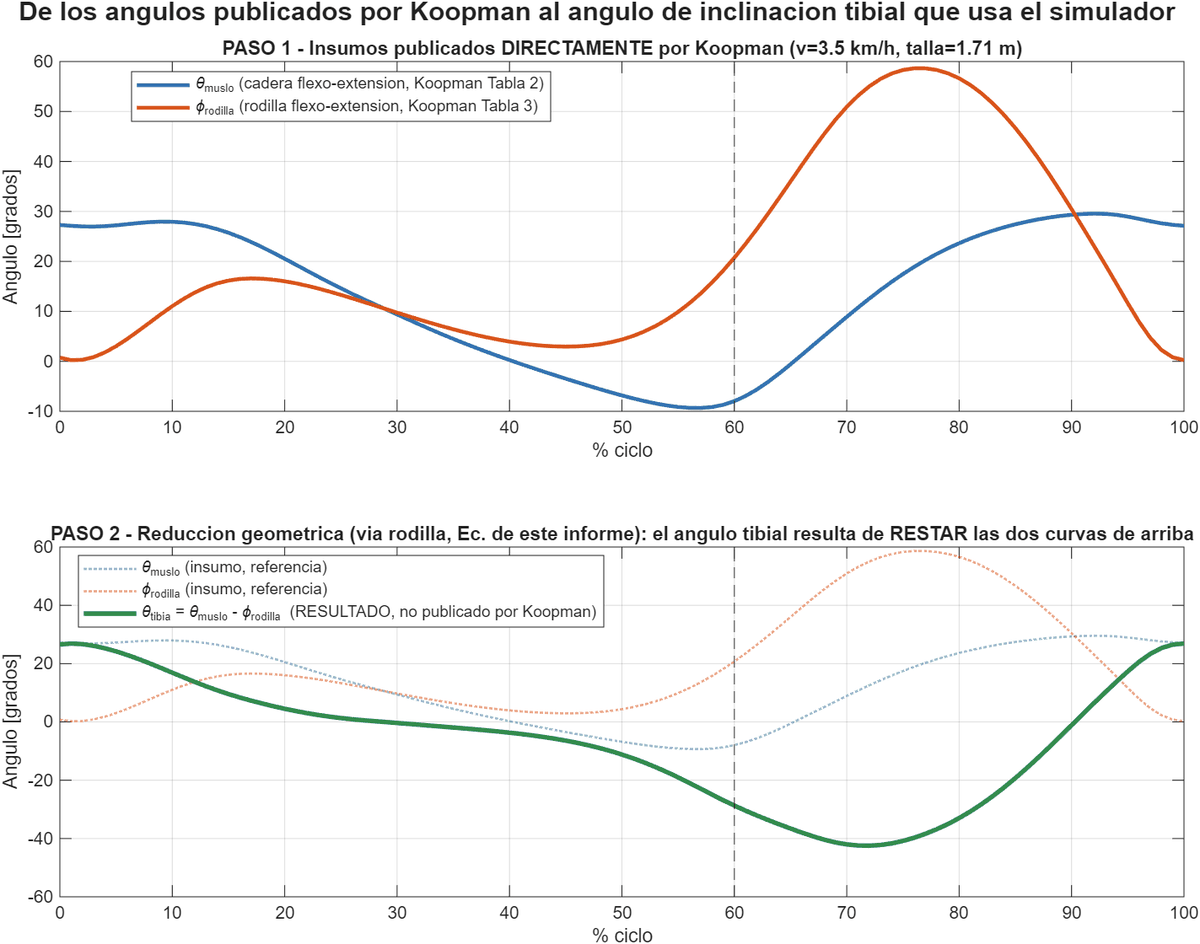
\includegraphics[width=0.85\textwidth]{figuras/23_reduccion_tibial_proceso_curvas_reales.png}
\caption{De los ángulos publicados por Koopman al ángulo tibial: arriba, $\theta_{muslo}(t)$ y $\varphi_{rodilla}(t)$ tal como salen de \texttt{Koopman2014\_Core.m} (Tablas 2 y 3 del paper); abajo, $\theta_{tibia}(t)=\theta_{muslo}(t)-\varphi_{rodilla}(t)$ (Ec.~\ref{eq:reduccion_via_rodilla}), verificado numéricamente contra la resta directa (error máximo $7\times10^{-15}$ grados, redondeo de punto flotante). Mismo caso que las Figuras~\ref{fig:koopman_4curvas} y~\ref{fig:salida_generador}.}
\label{fig:reduccion_tibial_proceso}
\end{figure}

Alternativa evaluada, vía tobillo (pie plano en apoyo, $\theta_{pie}=0$): $\theta_{tibia}=\theta_{pie}+\varphi_{tobillo}$.

\aporte{Comparadas ambas vías contra el registro de referencia del proyecto: vía rodilla $r=0.982$, vía tobillo $r=-0.435$ (signo contrario --- se aparta del movimiento real en el balanceo). Se usa vía rodilla en las dos fases del ciclo.}

\matlabtitle{las dos vías se calculan con la misma función (el signo es un parámetro explícito, no un supuesto oculto):}
\begin{lstlisting}
% via rodilla:
theta_tibia_via_rodilla = theta_muslo + signo_rodilla * phi_rodilla;  % signo_rodilla = -1
% via tobillo:
theta_tibia_via_tobillo = theta_pie   + signo_tobillo * phi_tobillo;  % signo_tobillo = +1
\end{lstlisting}
Cuál vía usar por candidato y por fase queda fijado en un único lugar del código (una tabla de decisión), no repetido en cada cálculo que la necesita --- si la regla cambia con nueva evidencia, cambia ahí una sola vez.

\section{Bases de datos de validación}
\label{sec:datos}

Regla de no circularidad (Sección~\ref{sec:contexto}): ninguna base usada para \emph{elegir} el modelo se reutiliza para \emph{reportar} qué tan bien funciona. Tabla~\ref{tab:bases_datos}.

\begin{table}[H]
\centering
\caption{Bases de datos usadas, en orden de exigencia creciente.}
\label{tab:bases_datos}
\small
\begin{tabular}{@{}p{2.6cm}p{1.0cm}p{2.6cm}p{2.6cm}p{4.0cm}@{}}
\toprule
Fuente & $n$ & Tipo de marcha & Antropometría & Rol \\
\midrule
Registro propio del proyecto & 1 & --- & --- & Primer cribado rápido \\
Winter~\cite{Winter2009} & 1 & marcadores de laboratorio & no documentada & Chequeo de forma \\
\emph{Maastricht}~\cite{Senden2024} & 246 & cinta, realidad virtual & de grupo (H, 18--29) & Selección, población grande \\
Ferber et al.~\cite{Ferber2024} & 40 & cinta & individual, medida & Selección, posición 3D real \\
\emph{Kuopio}~\cite{Lavikainen2024} & 15 (de 51) & overground real & individual, medida & Validación final y calibración \\
Camargo et al.~\cite{Camargo2021} & reservada & overground, escaleras & individual, medida & Examen final (no ejecutado) \\
\bottomrule
\end{tabular}
\end{table}

Solo \emph{Kuopio}~\cite{Lavikainen2024} combina marcha overground real y antropometría individual medida --- la única usada para validación final (Sección~\ref{sec:resultados}) y calibración LOSO (Sección~\ref{sec:calibracion}). 15 de 51 sujetos, 3 ensayos c/u.

\fuente{Contacto de talón detectado con el método cinemático de Zeni et al.~\cite{Zeni2008} (Kuopio no trae eventos precalculados).}

\aporte{Camargo et al.~\cite{Camargo2021} se reservó desde el diseño --- no participó en elegir ni calibrar el modelo. Se usaron 2 sujetos piloto solo para verificar la fórmula del Paso 1: tibia estimada 0.4428\,m vs.\ 0.446\,m medida (error $-0.7\,\%$). La comparación completa sigue pendiente (Sección~\ref{sec:limitaciones}).}

\section{Calibración por validación cruzada dejando-un-sujeto-fuera (LOSO)}
\label{sec:calibracion}

\aporte{Toda esta sección es calibración propia del proyecto --- Koopman et al.\ no reporta este defecto ni esta corrección.}

\subsection{El hallazgo}
\label{sec:hallazgo_calibracion}

Examinando sujeto por sujeto, la rodilla vertical predicha era más plana que la real: solo 51\,\% de la excursión real (el RMSE crudo no lo delataba porque la señal misma es pequeña). Causa: el ángulo de muslo de Koopman acierta la \emph{forma} ($r=0.971$) pero sobreestima la \emph{amplitud} 21\,\% ($32.5^\circ$ real vs.\ $39.2^\circ$ generado). El ángulo tibial, medido de forma independiente, dio una ganancia similar (0.811 vs.\ 0.769 del muslo) --- confirma un único defecto de amplitud (20--23\,\%), no uno distinto por eje.

\subsection{El método}
\label{sec:metodo_loso}

LOSO: para corregir un sujeto, los coeficientes se calculan solo con los otros 14, nunca con sus propios datos --- se repite por cada uno de los 15, evitando calibrar y evaluar con la misma observación.

\matlabtitle{el bucle de 15 pliegues (uno por sujeto):}
\begin{lstlisting}
for k = 1:numel(idx_ok)
    i = idx_ok(k);  otros = idx_ok(idx_ok ~= i);       % nunca el propio sujeto

    pm = polyfit(reshape(Thm_koop(otros,:),1,[]), reshape(Thm_real(otros,:),1,[]), 1);  % muslo
    pt = polyfit(reshape(Tht_koop(otros,:),1,[]), reshape(Tht_real(otros,:),1,[]), 1);  % tibia

    th_m_calibrado = deg2rad(pm(2)) + pm(1)*th_m;   % se aplica SOLO al sujeto i
    th_t_calibrado = deg2rad(pt(2)) + pt(1)*th_t;
end
\end{lstlisting}
Esto sirve para \emph{validar} (reportar los números de este informe: cada sujeto se predice "a ciegas"). Para \emph{producción} (generar la trayectoria de un sujeto nuevo, sin nadie que "dejar afuera"), se usa una única ganancia/offset ajustada con el conjunto agrupado completo --- ver nota de $N$ en Limitaciones.

\subsection{La corrección}
\label{sec:correccion_aplicada}

\begin{equation}
\theta_{final} = a + b \cdot \theta_{Koopman}
\label{eq:calibracion_afin}
\end{equation}

\begin{table}[H]
\centering
\caption{Coeficientes de la calibración afín, promedio de los 15 pliegues LOSO.}
\label{tab:coeficientes_calibracion}
\small
\begin{tabular}{@{}lrr@{}}
\toprule
Ángulo & Ganancia $b$ & Offset $a$ \\
\midrule
Muslo (rodilla) & 0.769 & $-2.69^\circ$ \\
Tibia (tobillo, ángulo tibial) & 0.811 & $-11.33^\circ$ \\
\bottomrule
\end{tabular}
\end{table}

Se aplica sobre el ángulo, \emph{antes} de convertirlo en posición por geometría (el Pipeline completo se detalla más adelante, Sección~\ref{sec:pipeline}) --- un primer intento calibrando la \emph{posición} ya calculada producía una curva "aplastada" sin sentido físico; se diagnosticó y se movió la corrección al lugar correcto: el ángulo, antes de la geometría.

\section{Pipeline de generación: de antropometría a trayectoria}
\label{sec:pipeline}

\aporte{Encadenar estos 5 pasos en una sola cadena reproducible, a partir de solo 3 datos de entrada (talla, masa, sexo) y combinando 4 fuentes independientes, es la construcción propia de este trabajo --- ninguna fuente define este pipeline completo.}

\textbf{Trazabilidad de las 3 entradas, resumen honesto antes de entrar al detalle paso a paso:} de las 3, solo la \textbf{talla} llega hasta el final de la trayectoria (Pasos 1, 2 y 4). La \textbf{masa} y el \textbf{sexo} entran a la función de contrato (\texttt{Generar\_Trayectoria.m} acepta ambos campos) pero \textbf{ningún paso de este pipeline los usa todavía} para calcular posición o ángulo --- la masa solo importa en el módulo aparte de predicción de fuerza (GRF --- fuera del alcance de este informe, documentado en \texttt{informe\_generador\_Luis.txt} Sección 9), y ahí una prueba explícita encontró que agregarla como tercera variable empeoraba la predicción con los datos disponibles (N=48) por sobreajuste, así que tampoco se usa ahí. El sexo no distingue ninguna de las fórmulas de los 4 candidatos evaluados --- limitación declarada, no un dato que "se perdió" en el camino.

\begin{table}[H]
\centering
\caption{Qué paso usa cada uno de los 3 datos de entrada.}
\label{tab:trazabilidad_entradas}
\small
\begin{tabular}{@{}lccc@{}}
\toprule
Paso & Talla & Masa & Sexo \\
\midrule
1. Antropometría segmentaria & Sí (Ec.~\ref{eq:l_muslo_tibia}) & No & No \\
2. Velocidad y tiempo de ciclo & Sí (Ecs.~\ref{eq:froude}, \ref{eq:step_ratio}) & No & No \\
3. Ángulos articulares por fase & Sí (heredada del Paso 2, vía $v$ y $l$) & No & No \\
4. Cadena cinemática (posición) & Sí (heredada, vía $L_{muslo}$, $L_{tibia}$, $v$) & No & No \\
5. Exportación & --- (solo formatea lo ya calculado) & No & No \\
\bottomrule
\end{tabular}
\end{table}

\subsection{Paso 1: antropometría segmentaria}
\label{sec:paso1}

\entradasalida{talla $H$ --- único dato de entrada real de este paso.}{$L_{muslo}$, $L_{tibia}$ (y $L_{pie}$, usado solo por el candidato Yun) --- las \textbf{longitudes} de segmento. $H$ se reutiliza tal cual en el \textbf{Paso 2}; $L_{muslo}$ y $L_{tibia}$ se usan en el \textbf{Paso 4} para la geometría. Las \emph{alturas} de cadera/rodilla/tobillo de más abajo son solo álgebra intermedia (de dónde salen las restas) --- el código no las calcula ni las guarda como variable; no son una salida real de este paso.}

\fuente{Drillis \& Contini 1966, fracciones de talla $H$, verificadas contra la Fig.\ 4.1 de Winter~\cite{Winter2009}.}

\begin{align*}
\text{cadera} &= 0.530\,H, &
\text{rodilla} &= 0.285\,H, &
\text{tobillo} &= 0.039\,H, &
\text{pie} &= 0.152\,H
\end{align*}
\begin{equation}
L_{muslo} = 0.245\,H \qquad L_{tibia} = 0.246\,H
\label{eq:l_muslo_tibia}
\end{equation}

Un dato medido siempre prevalece sobre uno estimado. No distingue por sexo (limitación declarada, a diferencia de de Leva~\cite{deLeva1996} para masa).

\textit{Trazabilidad de las 3 entradas en este paso: solo \textbf{talla} ($H$) entra --- las fracciones de Drillis \& Contini no distinguen por sexo, y la masa no interviene en ninguna longitud de segmento.}

\matlabtitle{la regla "medido gana sobre estimado" está codificada, no solo declarada --- nunca sobreescribe un campo que ya llegó medido:}
\begin{lstlisting}
if isfield(entrada, 'long_tibia_m') && ~isempty(entrada.long_tibia_m)
    out.fuente_tibia = 'medido';              % se deja tal cual vino
else
    out.long_tibia_m = 0.246 * H;             % Drillis & Contini 1966
    out.fuente_tibia = 'estimado_deLeva';
end
\end{lstlisting}

\aporte{Por qué importa esta regla en este proyecto específicamente: la fórmula por talla es un promedio poblacional de personas con las dos piernas intactas --- razonable para un sujeto sano (validado contra Camargo AB06, error 0.7\,\%), pero \textbf{no aplica a un muñón/tibia residual de un usuario transtibial}, cuya longitud depende del nivel de amputación de esa persona, no de su talla. En este ciclo del proyecto no se mide ningún segmento de ningún sujeto humano --- todas las validaciones (Camargo, Kuopio, Winter, Maastricht) usan la fórmula por talla porque son sujetos sin amputación. El campo \texttt{long\_tibia\_m} queda deliberadamente abierto y ya operativo para el día en que se mida el muñón real de un usuario de prótesis (una vez lo permita el protocolo de instrumentación): no hace falta tocar el código del generador, solo llenar ese campo con el dato medido.}

\subsection{Paso 2: velocidad de marcha y temporización del ciclo}
\label{sec:paso2}

\entradasalida{talla $H$ --- del \textbf{Paso 1}, reutilizada tal cual (este paso no recibe ninguna salida numérica \emph{nueva} del Paso 1, solo el mismo dato de entrada).}{velocidad $v$ y duración de ciclo $T_{ciclo}$. Las dos las necesita el \textbf{Paso 3}: las regresiones de Koopman (y de los otros candidatos) piden $v$ y talla como entrada.}

\fuente{$Fr=v^2/(gL)=0.25$ (velocidad "autoseleccionada"), Leurs et al.\ 2011~\cite{Leurs2011} --- verificado a texto completo y, además, la atribución de autor fue re-verificada contra Crossref el 28-ago-2026 (una referencia anterior lo atribuía a "Raichlen \& Pontzer 2011"; el hallazgo es correcto, el autor original estaba mal).}

\begin{equation}
v = \sqrt{Fr \cdot g \cdot L}, \qquad L = 0.530\,H
\label{eq:froude}
\end{equation}

\textbf{Aviso de notación --- dos variables que no deben confundirse:} la $L$ mayúscula de la Ec.~\ref{eq:froude} es la ``longitud de pierna'' de la literatura de Froude/marcha (altura de cadera, $0.530\,H$ --- la misma fracción de Drillis \& Contini del Paso 1, reutilizada aquí, no una constante nueva). No tiene relación con la $l$ minúscula que aparece en las fórmulas de Koopman (Ec.~\ref{eq:koopman_regresion} y la Ec.~\ref{eq:step_ratio} de abajo): ahí $l$ es directamente la talla corporal $H$, en la notación propia del paper (``$v$ represents walking-speed, $l$ body-height''). Son dos símbolos parecidos para dos roles distintos: $L$ solo se usa para estimar $v$ (fuera de Koopman); $l$ es un predictor dentro de las regresiones de Koopman (incluida la de $r_{paso}$).

\aporte{Con $v$ disponible, la duración de ciclo usa la Ec.\ 3 de Koopman et al.~\cite{Koopman2014} (su Tabla 5), reutilizada como reloj \emph{común a los tres candidatos} --- decisión propia, ninguna fuente lo especifica así.}

\fuente{Definición de $r_{paso}$ (``step-ratio''): el propio Koopman et al.\ la toma de Sekiya \& Nagasaki 1998 (citado dentro de Koopman 2014, no verificado a texto completo por separado en este proyecto) --- longitud de paso dividida entre frecuencia de paso, un cociente que esos autores encontraron aproximadamente constante en un rango amplio de velocidades de marcha:}
\begin{equation}
r_{paso} = \frac{\text{longitud de paso (m)}}{\text{frecuencia de paso (pasos/s)}} = \frac{1}{4}\cdot\frac{\text{longitud de zancada}}{\text{frecuencia de zancada}}
\label{eq:def_step_ratio}
\end{equation}

Como el propio Koopman explica, este cociente casi no depende de la velocidad --- por eso sirve como ``descriptor simple'' que sí se puede predecir con una regresión lineal en $v$ y $l$ (Tabla 5 del paper, Ec.~\ref{eq:step_ratio}):
\begin{align}
r_{paso} &= -0.532 + 0.020\,v + 0.47\,l \label{eq:step_ratio}\\
T_{ciclo} &= 2\sqrt{\dfrac{r_{paso}}{v/3.6}} \label{eq:tiempo_ciclo}
\end{align}

\aporte{De dónde sale la Ec.~\ref{eq:tiempo_ciclo}, paso a paso (álgebra directa desde la Ec.~\ref{eq:def_step_ratio}, no una fórmula arbitraria): si $v = \text{longitud de paso} \times \text{frecuencia de paso}$ (con $v$ en \textbf{m/s} aquí), despejando frecuencia de paso $=v/\text{longitud de paso}$, entonces $r_{paso} = \text{longitud de paso}/(v/\text{longitud de paso}) = \text{longitud de paso}^2/v$, de donde $\text{longitud de paso} = \sqrt{r_{paso}\cdot v}$. Un ciclo completo (zancada) son 2 pasos, así que $T_{ciclo} = 2/\text{frecuencia de paso} = 2\cdot\text{longitud de paso}/v = 2\sqrt{r_{paso}/v}$ (con $v$ en m/s) --- exactamente la Ec.~\ref{eq:tiempo_ciclo}. Lo único estimado por regresión es el valor de $r_{paso}$ (Ec.~\ref{eq:step_ratio}); el paso de $r_{paso}$ a $T_{ciclo}$ es cinemática exacta, no un segundo ajuste empírico.}

\textbf{De dónde sale el ``/3.6'' de la Ec.~\ref{eq:tiempo_ciclo}:} es solo conversión de unidades, no parte de la física. Koopman define $v$ en \textbf{km/h} para \emph{todas} sus tablas de regresión (``Speed is defined in kph''), así que la Ec.~\ref{eq:step_ratio} recibe $v$ en km/h para predecir $r_{paso}$. Pero la derivación de arriba ($T_{ciclo}=2\sqrt{r_{paso}/v}$) exige $v$ en \textbf{m/s} para que las unidades cuadren (si no, $r_{paso}$ tendría unidades de m$\cdot$s y dividir entre km/h no da segundos). $1\,\text{km/h} = 1/3.6\,\text{m/s}$, entonces $v_{\text{m/s}} = v_{\text{kph}}/3.6$ --- por eso el mismo número de velocidad aparece dos veces en la Ec.~\ref{eq:step_ratio}--\ref{eq:tiempo_ciclo}, primero tal cual (en kph, dentro de la regresión) y luego dividido entre 3.6 (convertido a m/s, dentro de la raíz).

Ciclo dividido 60\,\% apoyo / 40\,\% balanceo (estándar de la literatura). Advertencia activa: con $Fr=0.25$, $v$ supera el rango validado por Koopman (0.5--5\,km/h) para tallas $>1.48$\,m --- extrapolación conocida.

Ambas fórmulas se usan tal cual están publicadas, encadenadas: primero $v$, luego $T_{ciclo}$ con esa misma $v$. La del tiempo de ciclo se implementó una sola vez y se reutiliza para los tres candidatos evaluados (Sección~\ref{sec:busqueda}), sin duplicar el coeficiente en cada uno.

\aporte{Trazabilidad de las 3 entradas en este paso: \textbf{talla} entra dos veces con roles distintos ($L$ en la Ec.~\ref{eq:froude} para estimar $v$; $l$ en la Ec.~\ref{eq:step_ratio} para estimar $r_{paso}$ --- ver aviso de notación arriba). \textbf{Sexo y masa no entran} --- ninguna de las dos fórmulas de este paso las usa.}

\matlabtitle{velocidad y tiempo de ciclo, encadenados:}
\begin{lstlisting}
L = 0.530 * talla_m;                          % Ec. 5, longitud de pierna
v_ms = sqrt(Fr * g * L);                      % Ec. 4, Fr = 0.25

coef_step_ratio = [-0.532, 0.020, 0, 0.47];   % Koopman 2014, Tabla 5
step_ratio = coef_step_ratio(1) + coef_step_ratio(2)*v_kph ...
           + coef_step_ratio(3)*v_kph^2 + coef_step_ratio(4)*l_m;
tiempo_ciclo_s = 2 * sqrt(step_ratio / (v_kph/3.6));   % Ec. 3
\end{lstlisting}
Dispara una advertencia automática si $v$ cae fuera de 0.5--5\,km/h (rango validado por Koopman).

\subsection{Paso 3: ángulos articulares por fase}
\label{sec:paso3}

\entradasalida{$v$ y $T_{ciclo}$ --- del \textbf{Paso 2}. Talla $H$ --- del \textbf{Paso 1}, para la regresión de Koopman.}{las 4 curvas de ángulo de Koopman y, por reducción geométrica, $\theta_{muslo}(t)$ y $\theta_{tibia}(t)$ --- los dos ángulos que necesita el \textbf{Paso 4} para calcular posición.}

Con velocidad y talla ya fijas (Pasos 1 y 2), se reconstruyen las 4 curvas (Sección~\ref{sec:koopman}) y se obtiene el ángulo tibial con la Ec.~\ref{eq:reduccion_via_rodilla}. La Figura~\ref{fig:koopman_4curvas} muestra exactamente cuáles son esas 4 curvas, para un caso concreto (no un esquema).

\begin{figure}[H]
\centering
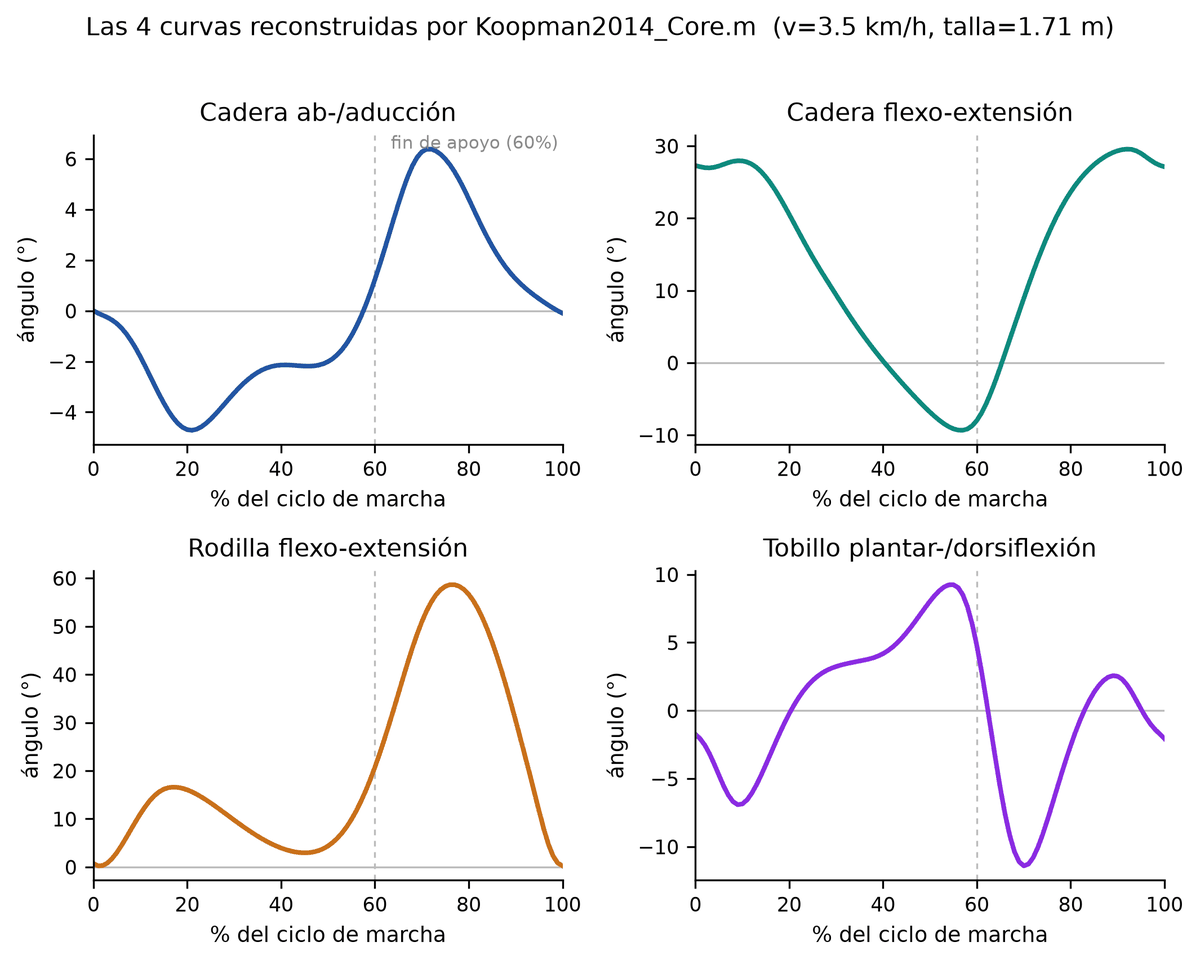
\includegraphics[width=0.92\textwidth]{figuras/13_koopman_4_curvas_reconstruidas.png}
\caption{Las 4 curvas que reconstruye \texttt{Koopman2014\_Core.m} para un caso concreto ($v$=3.5\,km/h, talla=1.71\,m): cadera ab-/aducción, cadera flexo-extensión, rodilla flexo-extensión, tobillo plantar-/dorsiflexión --- salida directa de las Tablas 1--4 (Sección~\ref{sec:koopman}), antes de cualquier reducción o calibración. La línea vertical marca el fin del apoyo (60\,\% del ciclo).}
\label{fig:koopman_4curvas}
\end{figure}

De esas 4, dos (cadera flexo-extensión y rodilla flexo-extensión) son las que entran a la Ec.~\ref{eq:reduccion_via_rodilla} para obtener el ángulo tibial --- la Figura~\ref{fig:reduccion_tibial} muestra qué segmentos y ángulos representa esa ecuación.

\begin{figure}[H]
\centering
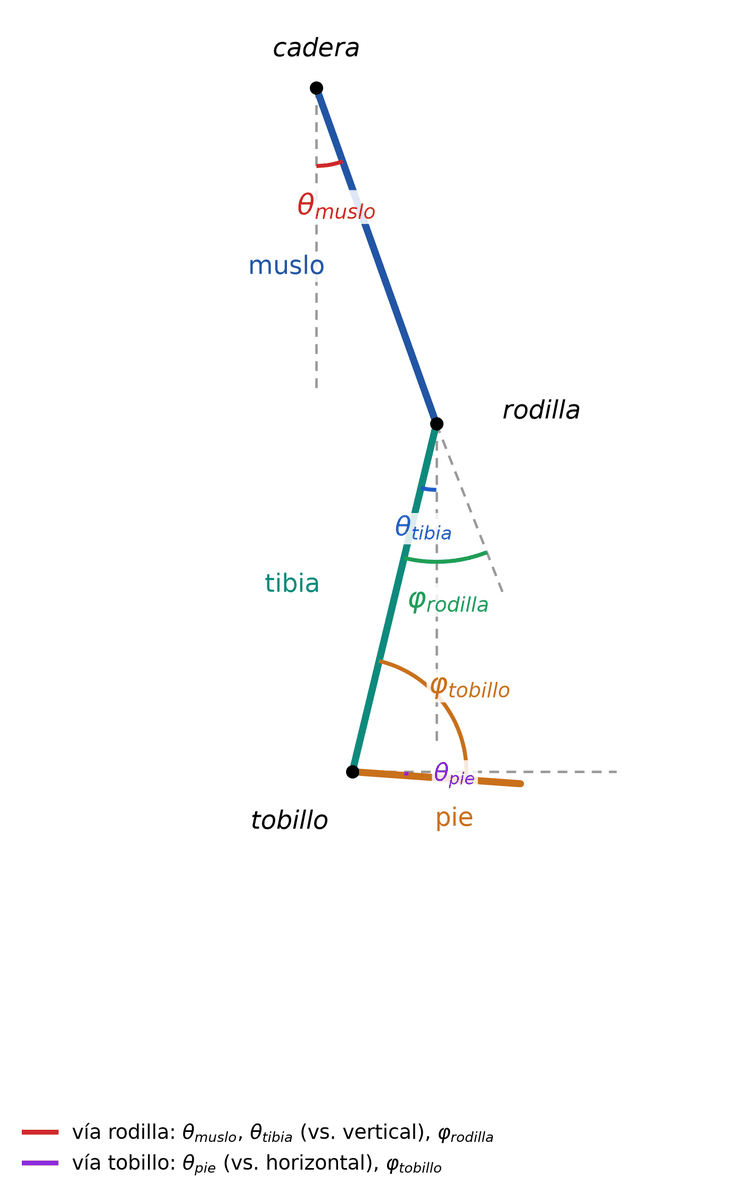
\includegraphics[width=0.55\textwidth]{figuras/12_reduccion_angulo_tibial_esquema.png}
\caption{Segmentos y ángulos de la reducción a ángulo de inclinación tibial (esquemático, no a escala; los valores de los ángulos dibujados son solo ilustrativos, no un caso numérico real). $\theta_{muslo}$ y $\theta_{tibia}$ se miden respecto a la vertical (líneas discontinuas en cadera y rodilla, misma convención que usa el simulador); $\theta_{pie}$ respecto a la horizontal (línea discontinua en el tobillo). $\varphi_{rodilla}$ y $\varphi_{tobillo}$ son los ángulos articulares relativos que sí publica Koopman. La vía rodilla (rojo/azul/verde) combina $\theta_{muslo}$ y $\varphi_{rodilla}$ (Ec.~\ref{eq:reduccion_via_rodilla}); la vía tobillo (púrpura/naranja) combina $\theta_{pie}$ y $\varphi_{tobillo}$ --- dos caminos geométricos independientes para llegar al mismo $\theta_{tibia}$, comparados en la Sección~\ref{sec:reduccion_tibial}.}
\label{fig:reduccion_tibial}
\end{figure}

\subsection{Paso 4: de ángulos a posición --- cinemática directa de péndulo doble}
\label{sec:paso4}

\entradasalida{$\theta_{muslo}(t)$, $\theta_{tibia}(t)$ --- del \textbf{Paso 3}. $L_{muslo}$, $L_{tibia}$ --- del \textbf{Paso 1}. $v$ --- del \textbf{Paso 2} (para la traslación horizontal de la cadera).}{posición $(x,y)$ de rodilla y tobillo en el tiempo --- la trayectoria misma, lo que exporta el \textbf{Paso 5}.}

\aporte{Reconstruido de cero el 30-ago-2026, reemplazando un primer modelo con conmutación explícita de fase (tobillo pivote fijo en apoyo, cadera pivote en balanceo, más un residuo empírico aditivo). Ese modelo anterior tenía una costura entre fases que producía discontinuidades reales de posición y velocidad. El modelo nuevo es cinemática DIRECTA de cadena abierta cadera$\to$rodilla$\to$tobillo (``péndulo doble''), UNA SOLA fórmula para todo el ciclo, sin conmutación de fase y sin ninguna corrección aditiva:}

\begin{equation}
x_k = x_h + L_{muslo}\sin\theta_{muslo},\qquad y_k = y_h - L_{muslo}\cos\theta_{muslo}
\label{eq:cadena_rodilla}
\end{equation}
\begin{equation}
x_a = x_k + L_{tibia}\sin\theta_{tibia},\qquad y_a = y_k - L_{tibia}\cos\theta_{tibia}
\label{eq:cadena_tobillo}
\end{equation}

donde $\theta_{muslo}$ y $\theta_{tibia}$ (vía rodilla) son los mismos ángulos del \textbf{Paso 3} --- esta etapa no cambia nada de la parte angular, solo cómo se convierte en posición.

\textbf{La cadera $(x_h,y_h)$ tiene dos componentes:}
\begin{equation}
x_h(t) = v\cdot t \qquad\text{(avance horizontal lineal, velocidad promedio constante)}
\label{eq:cadera_x}
\end{equation}
\begin{equation}
y_h(t) = y_0 - A\cos\!\left(\dfrac{4\pi t}{T_{ciclo}}\right),\quad A\approx2.25\,\text{cm}\ (\approx4.5\,\text{cm pico a pico})
\label{eq:cadera_y}
\end{equation}

\aporte{$A$ verificado contra literatura (Saunders, Inman \& Eberhart 1953, ``The Major Determinants in Normal and Pathological Gait''\cite{Saunders1953}: excursión vertical del centro de masa de $\sim$4--5\,cm pico a pico, confirmada en fuentes posteriores). La Ec.~\ref{eq:cadera_y} da, por construcción exacta, mínimos en $t=0\,\%$/$50\,\%$ del ciclo (contacto inicial de cada pie) y máximos en $t=25\,\%$/$75\,\%$ (medio apoyo) --- y CIERRA EL CICLO exactamente ($y_h(0\,\%)=y_h(100\,\%)$), a diferencia de un primer intento probado y descartado el mismo día (cadera anclada a la geometría de la pierna en el piso, alternando de pierna cada medio ciclo), que no cerraba el ciclo en el empalme.}

\matlabtitle{cinemática directa, una sola fórmula para todo el ciclo (Trayectoria\_Cadera\_Core.m + Cinematica\_DoblePendulo\_Core.m):}
\begin{lstlisting}
% cadera: avance lineal + oscilacion doble giba (Ecs. cadera_x, cadera_y)
Xh_cm = zancada_cm * (pct_ciclo/100);
Yh_cm = Y0_cm - A_cm*cos(4*pi*pct_ciclo/100);

% cadena directa cadera -> rodilla -> tobillo (Ecs. cadena_rodilla, cadena_tobillo)
Xk = Xh_cm + L1*sin(theta1);   Yk = Yh_cm - L1*cos(theta1);
Xa = Xk    + L2*sin(theta2);   Ya = Yk    - L2*cos(theta2);
\end{lstlisting}

Se construyó además una app interactiva (\texttt{App\_Animacion\_Cadera\_Rodilla\_Tobillo.m}) para explorar el modelo en vivo: talla editable, slider manual de \%ciclo, botón reproducir/pausar, mapa con la cadena + trayectoria punteada revelada progresivamente, y gráficas de desplazamiento normalizadas al punto inicial.

\textbf{Verificación:} (1) comportamiento físico correcto --- el tobillo despega y se levanta $\sim$7\,cm durante el balanceo, sin necesidad de imponer ninguna curva de elevación (Figura~\ref{fig:salida_generador}, Paso 5); (2) comparación DIRECTA, sin ninguna calibración, contra los 44 sujetos disponibles del \emph{Kuopio Gait Dataset} --- resultados completos en la Sección~\ref{sec:resultados_finales}.

\aporte{\textbf{Regla metodológica, fijada 31-ago-2026:} tanto la app como toda comparación contra \emph{Kuopio} en este informe reciben \textbf{solo la talla} como entrada --- masa/muslo/tibia/velocidad se ESTIMAN (Pasos 1--2), nunca se usa el valor real medido de cada sujeto, aunque \emph{Kuopio} lo tenga disponible. Es la única forma de que los números de esta sección sean comparables 1:1 con lo que la app le entrega a un usuario real, que solo mide la talla con una cinta métrica. Una primera pasada de esta validación (30--31-ago) sí usó antropometría/velocidad reales de \emph{Kuopio} para ajustar la corrección de posición --- eso hacía que el resultado no representara la app; se reajustó por completo con esta regla (\texttt{Refit\_CorreccionFinal\_TallaSola.m}, y luego \texttt{Ajustar\_Warp\_Temporal\_TallaSola.m} para el warp) antes de reportar los números de la Sección~\ref{sec:resultados_finales}.}

\aporte{\textbf{Bug de consistencia app--informe, encontrado y corregido 31-ago-2026:} la gráfica de desplazamiento de la app, con la corrección final activa, mostraba un valor final hasta \textbf{2.4--2.5\,cm distinto} del que reportan las Figuras~\ref{fig:rodilla_individual_pendulo_cal}/\ref{fig:tobillo_individual_pendulo_cal} para la MISMA talla. Causa: la corrección de posición (Ec.~\ref{eq:fourier_correccion}) es un ajuste afín $a(t)+b(t)\cdot crudo(t)$ que \emph{no} está forzado a pasar por 0 en $t{=}0$ --- forzarlo ya se había probado y revertido por empeorar el RMSEnorm (nota en \texttt{Correccion\_Posicion\_Suave\_PenduloDoble\_Core.m}). La gráfica de la app, sin embargo, SÍ re-normalizaba la curva corregida a 0 en $t{=}0$ antes de dibujarla --- cancelando exactamente ese término $a(0)$ que la corrección aprendió, y desalineándola de lo que valida este informe. \textbf{Corregido} en \texttt{App\_Animacion\_Cadera\_Rodilla\_Tobillo.m}: la gráfica de desplazamiento ahora usa la salida de la corrección \emph{tal cual}, sin renormalizar --- verificado numéricamente que, para la misma talla, la app y \texttt{Evaluar\_CorreccionFinal\_vs\_Kuopio.m} producen ahora la curva IDÉNTICA punto a punto (diferencia $<10^{-9}$\,cm). Las Figuras~\ref{fig:rodilla_individual_pendulo_cal}/\ref{fig:tobillo_individual_pendulo_cal} ya marcan el valor numérico del punto máximo de cada curva --- para verificar contra la app, ingresar la misma talla, activar ``Corrección final'', y comparar ese número con el valor final que muestra la gráfica de Desplazamiento X/Y de la app.}

Para un punto a distancia $d\leq L_{tibia}$ del tobillo (el sensor real de referencia no está en la rodilla anatómica sino a mitad de la tibia): misma geometría, reemplazando $L_{tibia}$ por $d$ en la Ec.~\ref{eq:cadena_tobillo}.

\subsection{Paso 5: exportación}
\label{sec:paso5}

\entradasalida{la trayectoria $(x,y,\text{ángulo})$ en el tiempo --- del \textbf{Paso 4}, el último que calcula algo nuevo.}{el archivo CSV en el formato exacto que ya lee el simulador --- de aquí en adelante nada se calcula, solo se formatea.}

\aporte{La trayectoria se exporta en el mismo formato, separador, paso de tiempo (0.01\,s) y resolución (0.0125\,cm X, 0.00625\,cm Y, $0.009^\circ$ ángulo) que el CSV real que el simulador ya lee.} La Figura~\ref{fig:salida_generador} muestra un ejemplo completo con el modelo del Paso 4 (péndulo doble + cadera oscilatoria) --- talla=1.71\,m (único dato de entrada real en este ejemplo), velocidad estimada por Froude (no medida) y muslo/tibia estimados por Drillis \& Contini --- regenerada 30-ago-2026 con el enfoque nuevo. Los paneles de Y (altura) están medidos respecto a la cadera ($y_h=0$, Ec.~\ref{eq:cadera_y}), no respecto al piso --- por eso rodilla y tobillo aparecen en valores negativos (cuelgan por debajo de la cadera). \textbf{Nota de integración (30-ago-2026):} \texttt{Escribir\_CSV\_Simulador.m} todavía lee del enfoque de posición ANTERIOR (el que este Paso 4 reemplaza) --- conectarlo al modelo nuevo es trabajo pendiente, no hecho en esta sesión.

\matlabtitle{cuantización + encabezado, verificado byte a byte contra el CSV real:}
\begin{lstlisting}
x_q = round(x_ctrl / 0.0125) * 0.0125;    % resolucion X
y_q = round(y_ctrl / 0.00625) * 0.00625;  % resolucion Y
ang_q = round(ang_ctrl / 0.009) * 0.009;  % resolucion angulo

% el archivo real de apoyo trae "Angulo_sagital apoyo" con ESPACIO, no
% guion bajo (inconsistencia real del dato, no de este escritor) - se
% replica tal cual para no romper lo que el simulador ya lee:
fprintf(fid, 'Tiempo_sagital_apoyo;Posicion_cm_X_apoyo;Posicion_cm_Y_apoyo;Angulo_sagital apoyo;;;\n');
fprintf(fid, '%.3f;%.4f;%.4f;%.4f;;;\n', t_ctrl(k), x_q(k), y_q(k), ang_q(k));
\end{lstlisting}
El CSV real no usa formato fijo (imprime "0" en vez de "0.0000") --- el valor tras el parseo es idéntico, aunque el texto no lo sea carácter por carácter.

\begin{figure}[H]
\centering
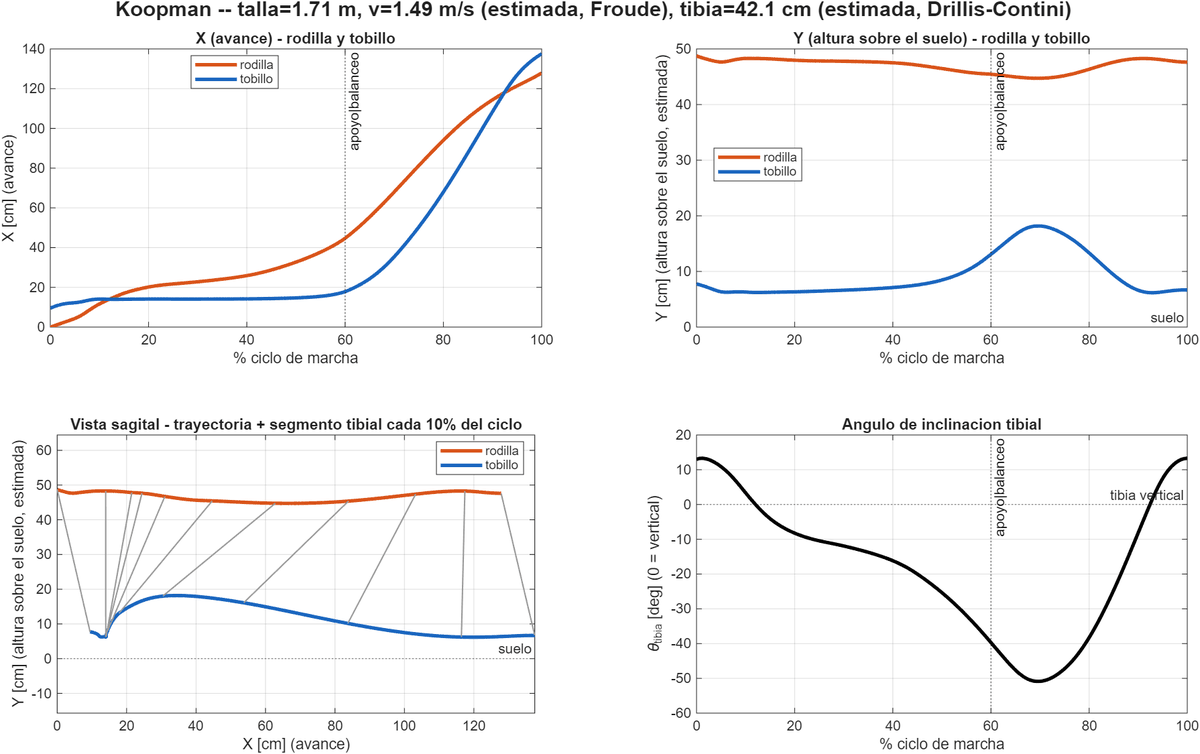
\includegraphics[width=0.9\textwidth]{figuras/05_generador_salida_koopman.png}
\caption{Ejemplo de salida del generador con el Paso 4 nuevo (talla 1.71\,m, Koopman crudo, sin calibrar): posición de rodilla/tobillo, cadena sagital completa, y ángulo tibial. Y medido respecto a la cadera, no al piso.}
\label{fig:salida_generador}
\end{figure}

\section{Resultados de validación}
\label{sec:resultados}

\subsection{Métricas}
\label{sec:metricas}

\begin{itemize}
    \item \textbf{$r$:} similitud de \emph{forma}, $[-1,1]$, independiente de escala/offset.
    \item \textbf{RMSE:} error cuadrático medio, unidades originales (°, cm).
    \item \textbf{RMSEnorm} \aporte{métrica propia}: RMSE normalizado por la variabilidad entre sujetos en cada instante del ciclo, comparable entre segmentos/estudios:
\end{itemize}

\begin{equation}
\mathrm{RMSEnorm} = \sqrt{\dfrac{1}{N}\sum_{i=1}^{N}\left(\dfrac{\theta_{pred}(i)-\theta_{real}(i)}{\mathrm{SD}_{entre\ sujetos}(i)}\right)^{2}}
\label{eq:rmsenorm}
\end{equation}

Escala: $<1$ Excelente, $<1.5$ Bueno, $<2$ Aceptable, $>2$ Deficiente.

\subsection{Resultados finales por segmento}
\label{sec:resultados_finales_top}

\subsubsection{Corrección de posición: warp temporal en $X$, Fourier en $Y$}
\label{sec:retrocesos_x}

Esta corrección se aplica DESPUÉS de generar la posición por péndulo doble con el ángulo YA calibrado (LOSO, Sección~\ref{sec:calibracion} + Paso 4, Sección~\ref{sec:paso4}) --- nunca antes. Ese crudo (ángulo calibrado + geometría) ya tiene buena \emph{forma} pero RMSE grande frente al dato real, así que se corrige por eje, con el método que corresponde a la naturaleza física de cada uno:

\begin{itemize}
\item \textbf{$X$ (avance):} físicamente monótono creciente (Ec.~\ref{eq:cadera_x}) --- caminando hacia adelante, un paso no retrocede. Se corrige con una \textbf{deformación de tiempo} (\emph{time-warp}) en vez de una corrección de amplitud, precisamente para no poder romper esa monotonía.
\item \textbf{$Y$ (vaivén vertical):} oscila libremente, sin monotonía que proteger --- se corrige con una serie de Fourier, punto a punto. \textbf{Se probó también el warp en $Y$ (mismo modelo vigente: Ec.~\ref{eq:warp_ode} + afín CONSTANTE, sin covariable) y perdió claramente contra Fourier} (LOSO real $N$=44: Rodilla Y, RMSEnorm 0.89 Fourier vs.\ 1.62 warp; Tobillo Y, 0.92 vs.\ 1.82) --- no es una elección solo argumentada, se descartó con evidencia: el warp únicamente reordena el tiempo, no puede corregir que el pico de $Y$ esté sobre/subestimado en un tramo específico, que es justo el defecto que tiene $Y$ (Figura~\ref{fig:rodilla_desglose}).
\end{itemize}

\textbf{La ecuación diferencial (warp de $X$ --- SOLO $X$, rodilla y tobillo; $Y$ nunca pasa por esta ecuación, sigue por Fourier más abajo):} se construye en 4 pasos, cada uno resolviendo por qué el paso anterior no basta.

\begin{enumerate}
\item \textbf{Qué se necesita:} una función $corregido(t)$ tal que $\frac{d(corregido)}{dt}\geq0$ siempre --- eso es, literalmente, la definición de "no retrocede".
\item \textbf{Por qué corregir la \emph{amplitud} (como Fourier, Ec.~\ref{eq:fourier_correccion}) no sirve para esto:} en $corregido(t)=a(t)+b(t)\cdot crudo(t)$, la derivada es $a'(t)+b'(t)\cdot crudo(t)+b(t)\cdot crudo'(t)$ --- una suma de 3 términos con signos independientes. Nada obliga a que esa suma sea $\geq0$ en todo $t$, y de hecho no lo es: se probó Fourier también en $X$ (misma Ec.~\ref{eq:fourier_correccion} que usa $Y$, coeficientes de producción con los 44 sujetos) y produjo retrocesos donde el crudo no los tenía --- verificado para talla=1.70\,m: rodilla, de 0/100 a 4/100 pasos negativos; tobillo, de 11/100 a 22/100 --- el mismo defecto que motivó cambiar de familia de corrección para $X$.
\item \textbf{La idea: corregir \emph{cuándo} ocurre cada valor, no \emph{cuánto} vale.} Si en vez de tocar la amplitud se define $corregido(t)=crudo(\tau(t))$ para alguna función de tiempo $\tau$, la derivada es $crudo'(\tau(t))\cdot\tau'(t)$ (regla de la cadena) --- un producto de 2 términos, no una suma de 3. Si $crudo$ ya es monótono ($crudo'\geq0$, cierto para rodilla/tobillo X dentro del rango validado, Sección~\ref{sec:robustez_warp}) y se logra que $\tau'(t)\geq0$ \textbf{siempre}, el producto completo queda $\geq0$ siempre --- monotonía garantizada por construcción, no por casualidad del ajuste.
\item \textbf{Cómo garantizar $\tau'(t)\geq0$ siempre, para cualquier coeficiente que salga del ajuste:} en vez de pedirle al optimizador que respete una restricción de desigualdad (que puede fallar numéricamente o quedar justo en el borde), se parametriza $\tau'(t)$ como una \textbf{exponencial} de una función libre $g(t)$:
\begin{equation}
\frac{d\tau}{dt} = w(t) = e^{g(t)} > 0 \quad \text{siempre, para CUALQUIER $g(t)$ real}, \qquad \tau(0) = 0
\label{eq:warp_ode}
\end{equation}
con $g(t)$ una serie de Fourier de $K_w$ armónicos, sin término constante (se cancela con la normalización de cierre de abajo, Ec.~\ref{eq:cierre_tau}). Como $e^x>0$ para \emph{cualquier} $x$ (no hace falta acotar ni restringir $g$), $\tau(t)$ queda estrictamente creciente sin importar qué coeficientes encuentre el ajuste --- la garantía viene de la forma exponencial, no del resultado del ajuste.
\end{enumerate}

\textbf{Resolver la ecuación:} es una ODE de primer orden ya separada ($d\tau/dt$ no depende de $\tau$, solo de $t$), así que se resuelve por cuadratura directa (integral acumulada, \texttt{cumtrapz} en el código) en vez de un solver iterativo tipo \texttt{ode45}:
\begin{equation}
\tau_{bruto}(t) = \int_0^t e^{g(s)}\,ds, \qquad \tau(t) = \tau_{bruto}(t)\cdot\frac{100}{\tau_{bruto}(100)}
\label{eq:cierre_tau}
\end{equation}
el reescalado final garantiza $\tau(100)=100$ exacto --- el warp respeta el mismo ciclo de 0 a 100\,\% que todo lo demás del proyecto, sin necesitar una restricción aparte en el ajuste.

\aporte{\textbf{Esto sigue siendo una CORRECCIÓN, no un generador independiente:} $\tau(t)$ es solo una función de tiempo --- \texttt{Warp\_Temporal\_Core.m} no produce ninguna curva de posición por sí sola. La Ec.~\ref{eq:warp_afin} opera reevaluando el \emph{mismo} $crudo(\cdot)$ que ya entrega el pipeline existente (Koopman calibrado + \texttt{Cinematica\_DoblePendulo\_Core.m}, Sección~\ref{sec:paso4}) en los tiempos $\tau(t)$ en vez de en $t$ --- no hay ninguna otra fuente de datos.}

\textbf{El afín (constante, garantiza monotonía en talla):}
\begin{equation}
corregido(t) = a_0 + b_0\cdot crudo(\tau(t))
\label{eq:warp_afin}
\end{equation}
$a_0,b_0$ son constantes \emph{globales} (no dependen de \%ciclo ni de talla/velocidad). Con $b_0>0$ (verificado, Sección~\ref{sec:resultados_finales}) no pueden introducir retrocesos locales, y --- como $crudo(100\,\%)$ es monótono en talla por geometría pura ($r=1.000$, la talla determina $L_{muslo}$, $L_{tibia}$ y la zancada) --- la composición $a_0+b_0\cdot crudo$ queda \textbf{garantizada monótona en talla también}: a mayor talla, igual o mayor avance, siempre.

\aporte{\textbf{¿Por qué no depende de velocidad, si se pidió explícitamente que dependiera de otra entrada derivada de la talla?} Se probó (Sección~\ref{sec:resultados_finales}): un afín $\alpha(v)=a_0+a_1v$, $\beta(v)=b_0+b_1v$ SÍ reduce el RMSEnorm (de 1.10/1.17 a 0.96/0.98) --- pero a costa de la monotonía: el avance real al 100\,\% del ciclo no correlaciona con la talla dentro de los 44 sujetos de \emph{Kuopio} ($r=-0.01$), así que el ajuste de mínimos cuadrados aprendía una $\beta(v)$ que \emph{cancelaba} la escala natural con talla del crudo --- el resultado quedaba casi constante entre tallas, y en algún caso un sujeto más bajo terminaba con más avance que uno más alto. Se probó también talla como covariable de $\alpha$ con la restricción $a_1\geq0$ (que hubiera preservado la monotonía) --- el ajuste convergió exactamente a $a_1=0$: \textbf{no existe ninguna covariable derivada de la talla que mejore el ajuste sin romper el orden físico}. Se prefirió la versión constante: el costo en RMSE (en cm) es despreciable (11.4 vs 11.5\,cm rodilla, 9.5 vs 9.5\,cm tobillo) y a cambio se gana una garantía física, no solo estadística.

\textbf{Por qué es válido imponer esta restricción aunque los 44 sujetos individuales de \emph{Kuopio} no la cumplan siempre:} que el avance real no correlacione con la talla en esta muestra es \emph{ruido individual esperado} --- cada persona elige su velocidad de marcha cómoda por razones propias (condición física, hábito, preferencia), no solo por su estatura. El generador no busca replicar el ruido de un sujeto específico; busca producir, para un usuario nuevo, una trayectoria que respete el principio biomecánico general de que una pierna más larga permite --- a igual esfuerzo relativo --- una zancada más larga (el mismo principio que ya sostiene la Ec.~\ref{eq:froude}, Froude). Imponer esa restricción como prior de diseño, en vez de dejar que el ajuste absorba el ruido de la muestra, es una decisión metodológica defendible, no una que se esconda.}

\textbf{La corrección de $Y$ (Fourier):}
\begin{equation}
corregido(t) = a(t) + b(t)\cdot crudo(t), \qquad a(t) = \sum_{k=0}^{K} \big[a_{c,k}\cos(2\pi k t/100) + a_{s,k}\sin(2\pi k t/100)\big],\ b(t) \text{ análogo}
\label{eq:fourier_correccion}
\end{equation}
lineal en sus coeficientes --- se resuelve por mínimos cuadrados ordinarios. $K$=14 (barrido LOSO real, meseta estable desde $K\approx$12--14).

\aporte{\textbf{¿Es el warp un aporte propio, o una técnica ya publicada?} El principio general --- deformar el \emph{tiempo} de una curva en vez de su \emph{amplitud} para alinearla con una referencia --- es un área establecida de estadística funcional (\emph{curve registration}/\emph{dynamic time warping}, ver p.\,ej.\ Ramsay \& Silverman, \emph{Functional Data Analysis}). No se inventó la idea desde cero. Lo propio de este trabajo: (1) la formulación específica $d\tau/dt=e^{g(t)}$ con $g$ en base de Fourier; (2) el diagnóstico que motivó buscar esta familia --- que el problema de $X$ es de \emph{monotonía}, no solo de precisión; (3) verificar explícitamente, probando y descartando alternativas con covariables, que ninguna entrada derivada de la talla mejora el ajuste sin romper la monotonía --- así que el afín se deja constante a propósito, no por omisión; y (4) aplicar métodos \emph{distintos} a $X$ y a $Y$ según cada uno necesite o no la garantía de monotonía.}

\textbf{Número de armónicos del warp ($K_w$):} barrido LOSO real, $N$=44 --- meseta plana desde $K_w$=2 hasta $K_w$=12, verificado con el afín dependiente de velocidad (etapa de búsqueda, antes de fijar la versión constante) --- $K_w$ gobierna la suavidad de $\tau(t)$ (Ec.~\ref{eq:warp_ode}), un parámetro independiente de si el afín depende o no de una covariable, así que la elección se mantiene. \textbf{Se fija $K_w$=2} (el más simple que ya alcanza la meseta).

\textbf{Resultado (LOSO real, $N$=44, solo talla):} Rodilla X $r$=0.999/RMSEnorm=1.10/\textbf{0 retrocesos}; Tobillo X $r$=0.999/RMSEnorm=1.17/\textbf{0 retrocesos} --- ambos Bueno, sin retrocesos garantizados por construcción matemática (Ec.~\ref{eq:warp_ode}) Y monótonos en talla garantizados (Ec.~\ref{eq:warp_afin}, $b_0>0$), no por casualidad de un ajuste.

\subsubsection{Robustez: qué pasa dentro y fuera del rango validado}
\label{sec:robustez_warp}

\aporte{La garantía de "cero retrocesos" de la Ec.~\ref{eq:warp_ode} es matemática, pero \textbf{tiene una condición implícita que hay que verificar, no asumir}: la composición $a_0+b_0\cdot crudo(\tau(t))$ solo hereda la monotonía de $\tau(t)$ si (a) $b_0>0$ (verificado: $b_0$=0.664 rodilla, 0.636 tobillo, Sección~\ref{sec:resultados_finales}) y (b) $crudo(\cdot)$ en sí mismo ya era monótono \emph{antes} de aplicar el warp --- el warp reordena \emph{cuándo} ocurre cada valor de $crudo$, pero no puede eliminar una bajada que el propio $crudo$ ya tenía. Como $a_0,b_0$ son constantes fijas (no dependen de talla ni velocidad), la garantía de monotonía --- tanto en el tiempo (Ec.~\ref{eq:warp_ode}) como en la talla (por $b_0>0$ y $crudo(100\,\%)$ monótono en talla, $r$=1.000) --- aplica para \textbf{cualquier} talla que la app permita, no solo dentro de un rango de velocidad. Se verificó igual con un barrido de talla, no se dio por sentado.}

\textbf{Dentro del rango validado (161--186.6\,cm, mismo rango de los 44 sujetos de \emph{Kuopio}):} barrido fino cada $\approx$5\,mm (52 tallas) --- \textbf{0 fallos, 0 retrocesos en las 52} (rodilla y tobillo X). La garantía matemática se cumple exactamente donde se necesita.

\textbf{Fuera del rango (extremos permitidos por la app, 130--210\,cm):}

\begin{table}[H]
\centering
\caption{Retrocesos en tobillo X, dentro y fuera del rango validado --- CRUDO (antes de cualquier corrección) vs.\ HÍBRIDO (warp + afín constante).}
\label{tab:robustez_fuera_rango}
\small
\begin{tabular}{@{}rrrr@{}}
\toprule
Talla (cm) & $v$ (m/s) & Retrocesos CRUDO & Retrocesos HÍBRIDO \\
\midrule
130 (fuera, corto) & 1.30 & 9/100 & 4/100 \\
140 (fuera, corto) & 1.35 & 7/100 & 3/100 \\
150 (fuera, corto) & 1.40 & 6/100 & 2/100 \\
155 (fuera, corto) & 1.42 & 5/100 & 2/100 \\
161 (borde validado) & 1.45 & 1/100 & 0/100 \\
165 (dentro) & 1.46 & 0/100 & 0/100 \\
186.6 (borde validado) & 1.56 & 0/100 & 0/100 \\
190--210 (fuera, alto) & 1.57--1.65 & 0/100 & 0/100 \\
\bottomrule
\end{tabular}
\end{table}

\textbf{Diagnóstico:} para tallas por debajo del rango validado ($<$161\,cm, velocidad estimada $<$1.45\,m/s), el geométrico CRUDO del tobillo (péndulo doble + Koopman, \emph{antes} de cualquier corrección) empieza a tener retrocesos propios (hasta 9/100 en el extremo de 130\,cm) --- es un defecto del \textbf{modelo geométrico}, no de la corrección. El warp \textbf{nunca lo empeora} (consistente con la Ec.~\ref{eq:warp_ode}: no puede introducir retrocesos nuevos) y en la práctica lo \textbf{reduce ligeramente}, pero no lo elimina del todo porque no puede eliminar algo que ya estaba en el crudo. Para tallas por encima del rango (hasta 210\,cm, el máximo de la app) no aparece ningún retroceso, ni en crudo ni corregido.

\textbf{Conclusión práctica:} la corrección híbrida es segura para cualquier talla que la app permita --- \emph{nunca empeora} el retroceso frente al crudo --- pero la garantía de \emph{cero} retrocesos absoluto solo está demostrada y confirmada dentro de 161--186.6\,cm. La app ya avisa cuando la talla ingresada cae fuera del rango validado (Sección~\ref{sec:paso4}).

\subsubsection{¿Cuánto pesa la corrección frente a la geometría?}
\label{sec:peso_correccion_posicion}

\aporte{Si la corrección pesara más que la geometría que corrige, el resultado ya no sería ``péndulo doble corregido'' sino, en la práctica, ``\emph{Kuopio} con un poco de péndulo encima''. Se midió, dentro del rango de talla validado (161--186.6\,cm, $N$=44) --- descomponiendo la curva final en geometría sola (crudo) y corrección sola (delta = corregido $-$ crudo), Figura~\ref{fig:peso_correccion_posicion}.}

\begin{table}[H]
\centering
\caption{Rango de movimiento (ROM) aportado por la geometría (crudo) frente a la corrección (delta), medias $N$=44.}
\label{tab:peso_correccion_posicion}
\small
\begin{tabular}{@{}lrrr@{}}
\toprule
Curva & ROM geometría (cm) & ROM corrección (cm) & Corrección / geometría \\
\midrule
Rodilla X & 121.9 & 18.4 & \textbf{15\,\%} \\
Rodilla Y & 7.3 & 6.2 & \textbf{86\,\%} \\
Tobillo X & 122.1 & 21.3 & \textbf{17\,\%} \\
Tobillo Y & 15.9 & 9.9 & \textbf{62\,\%} \\
\bottomrule
\end{tabular}
\end{table}

\textbf{En $X$ la geometría manda} (péndulo doble + avance de cadera explican 83--85\,\% del recorrido; la corrección es un ajuste fino, $<$20\,\%) --- \textbf{en $Y$ la corrección hace la mayor parte del trabajo} (62--86\,\%), porque el movimiento vertical real en sí es chico (7--16\,cm de ROM). \textbf{Lectura honesta:} no debe afirmarse que ``el péndulo doble predice el desplazamiento vertical'' --- lo predice razonablemente en \emph{forma}, pero la magnitud final en $Y$ depende en buena parte de la corrección. En $X$ sí es correcto decir que el modelo (cadera + péndulo) domina.

\begin{figure}[H]
\centering
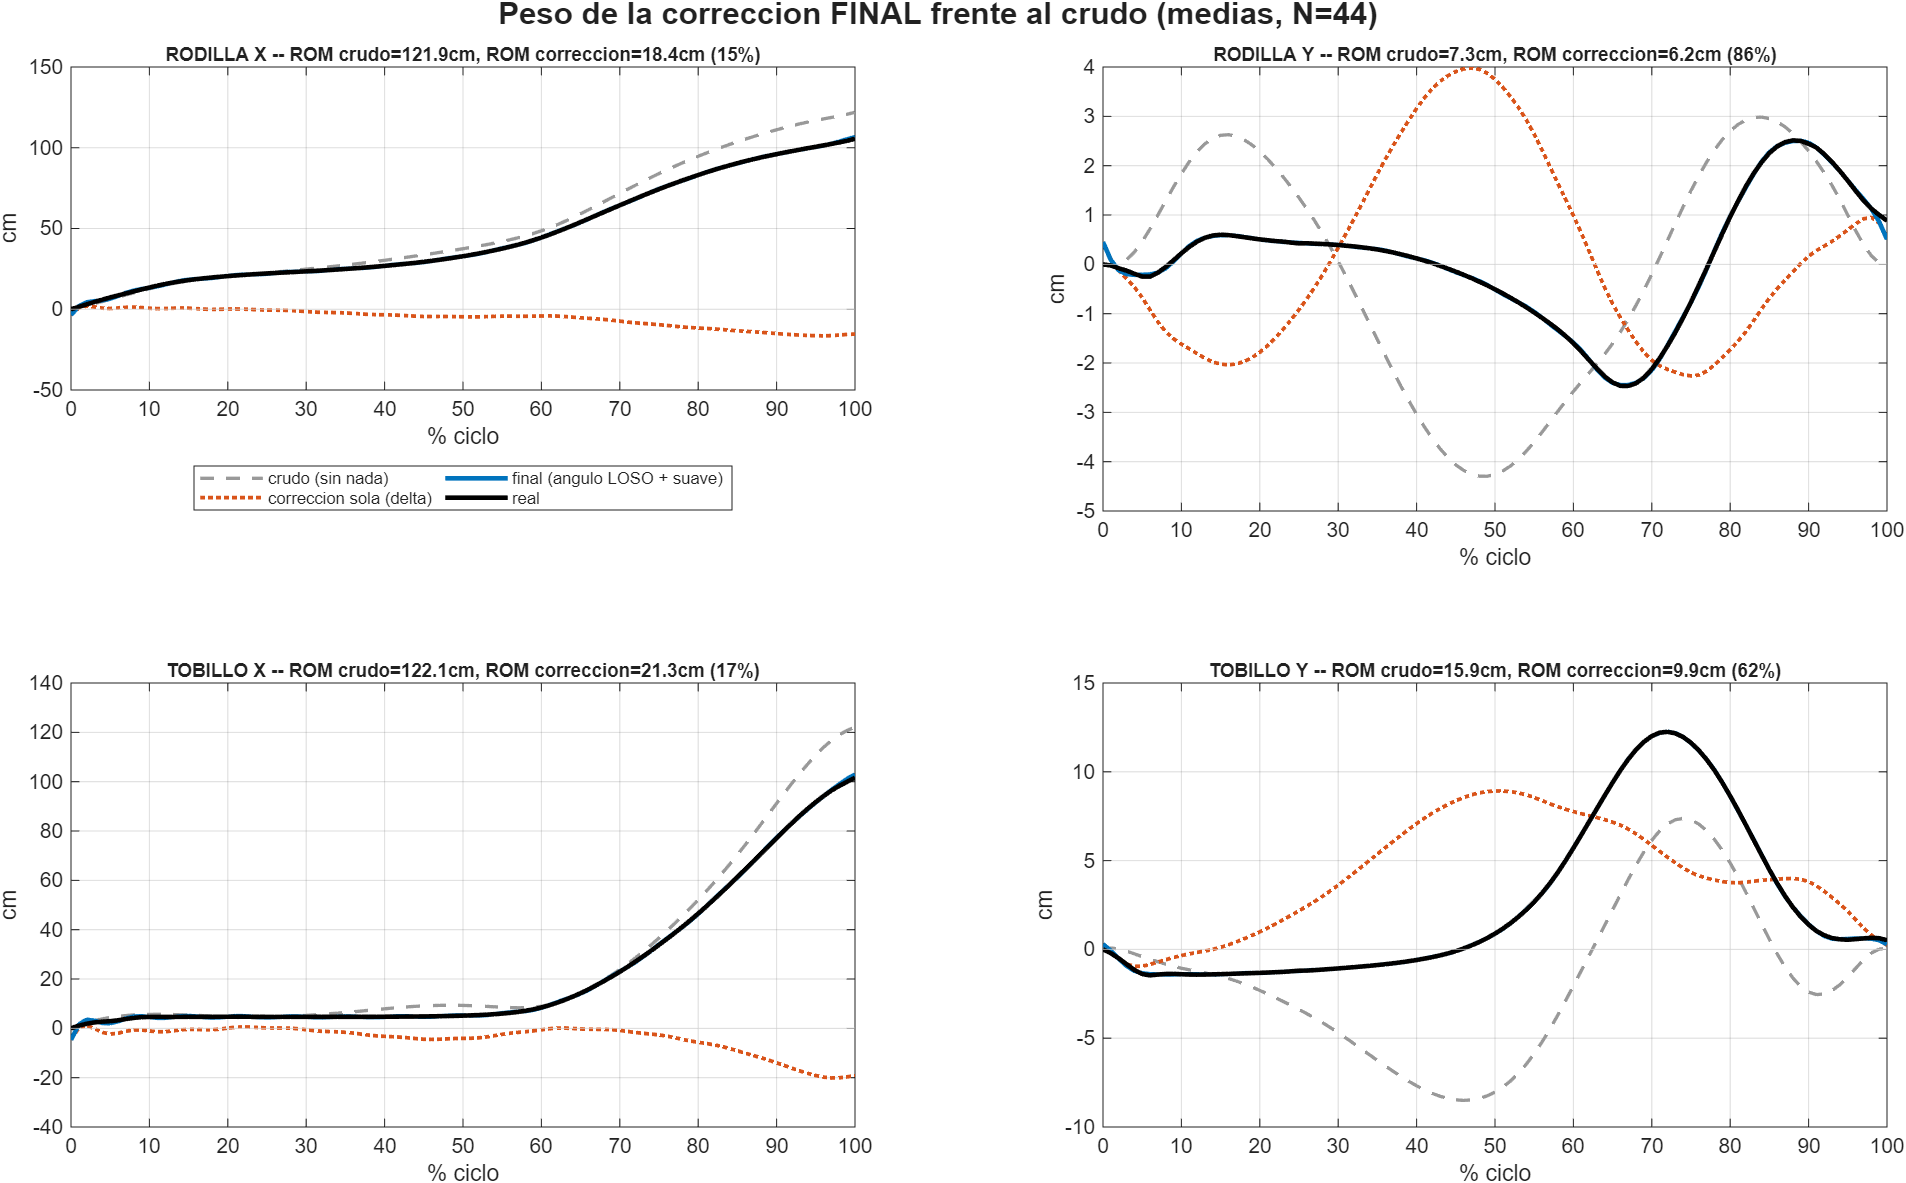
\includegraphics[width=0.95\textwidth]{figuras/26_peso_correccion_posicion.png}
\caption{Descomposición de la curva final en geometría sola (crudo, gris discontinuo), corrección sola (delta, punteado naranja) y curva final corregida (azul) vs.\ real (negro) --- 44 sujetos, curvas media, dentro del rango de talla validado.}
\label{fig:peso_correccion_posicion}
\end{figure}

\begin{figure}[H]
\centering
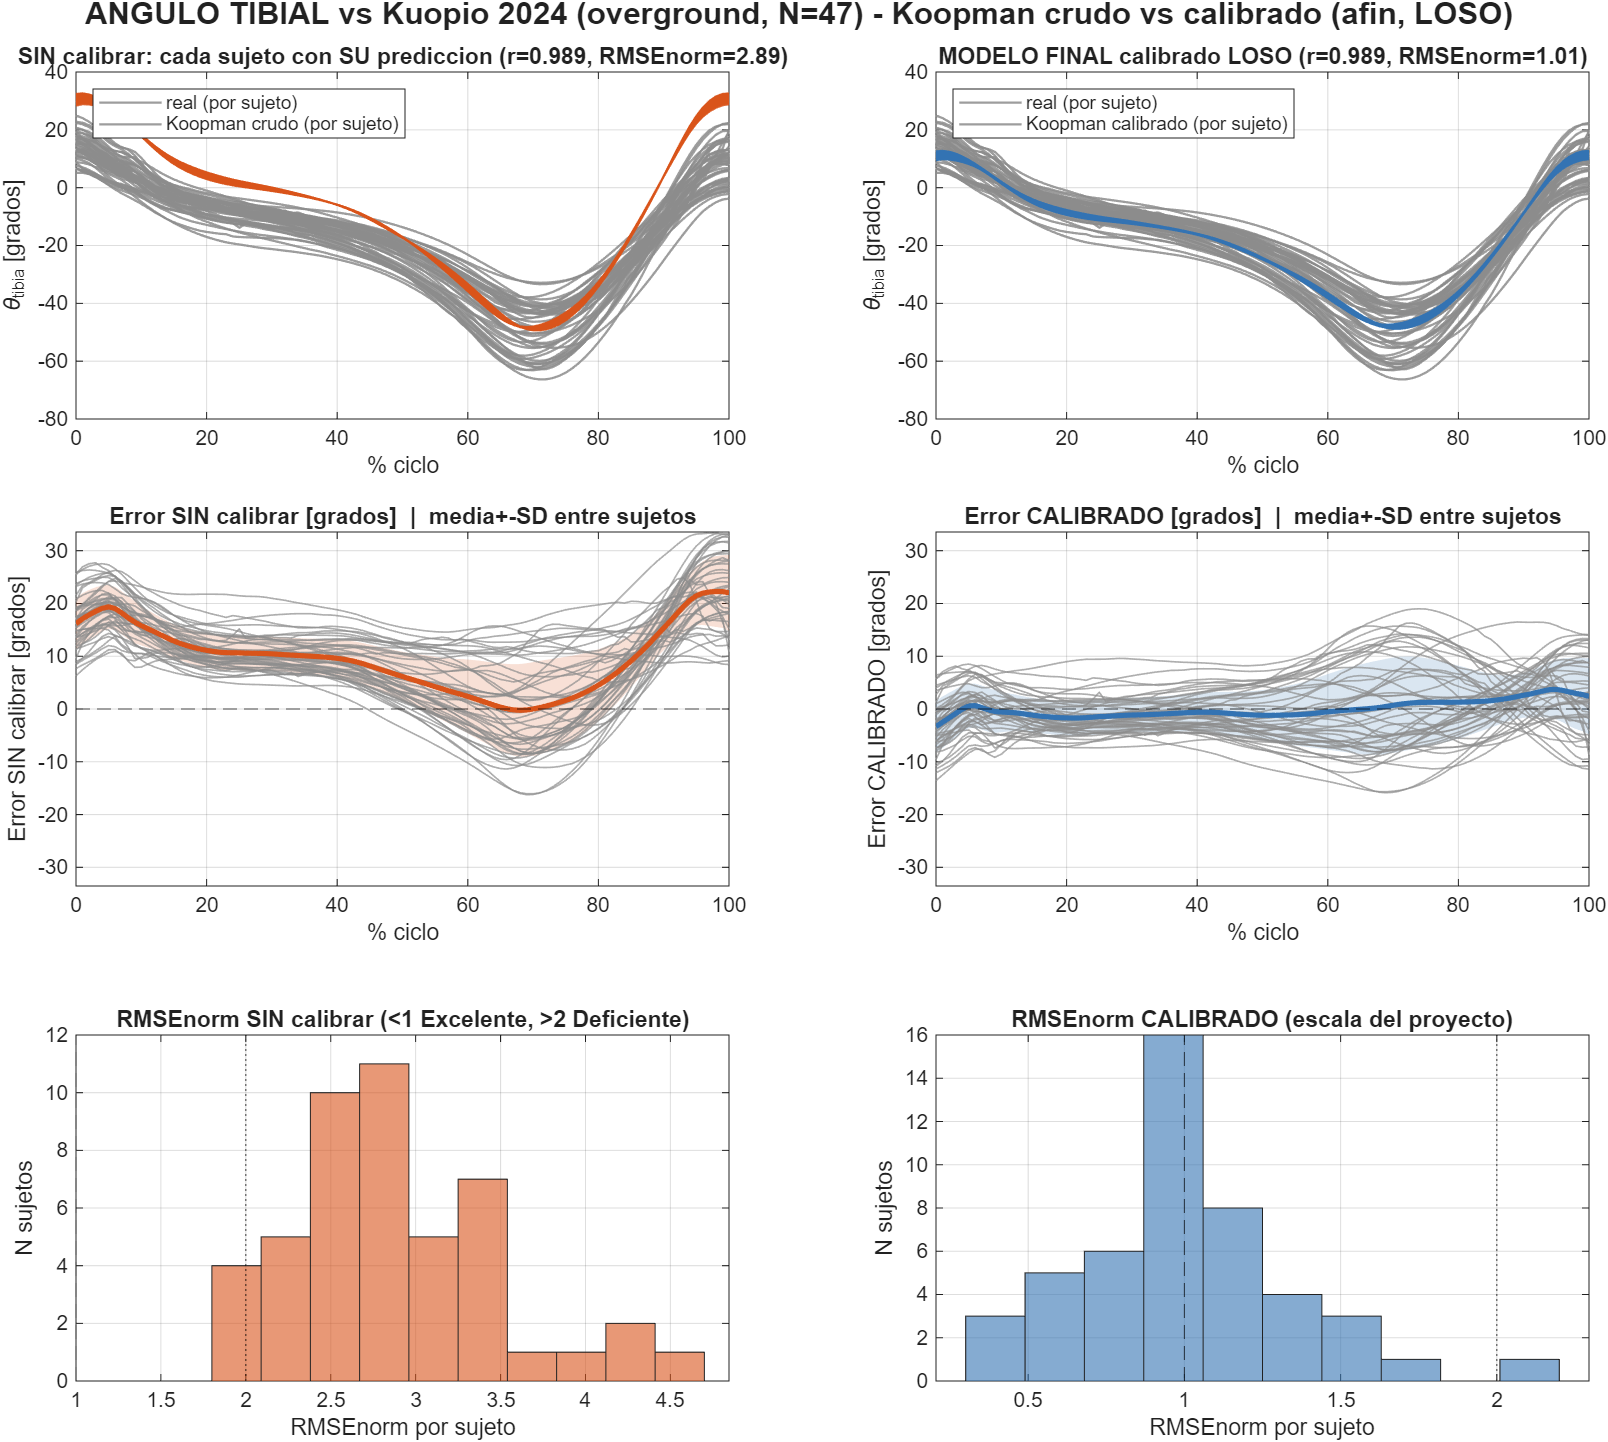
\includegraphics[width=0.8\textwidth]{figuras/10_angulo_tibial_vs_kuopio_grupo.png}
\caption{Ángulo tibial, sin calibrar vs.\ calibrado (LOSO), $N$=47, SOLO TALLA como entrada. El histograma muestra el corrimiento de RMSEnorm de "Deficiente" a "Bueno"/"Excelente" en casi todos los sujetos.}
\label{fig:tibial_grupo}
\end{figure}

\begin{figure}[H]
\centering
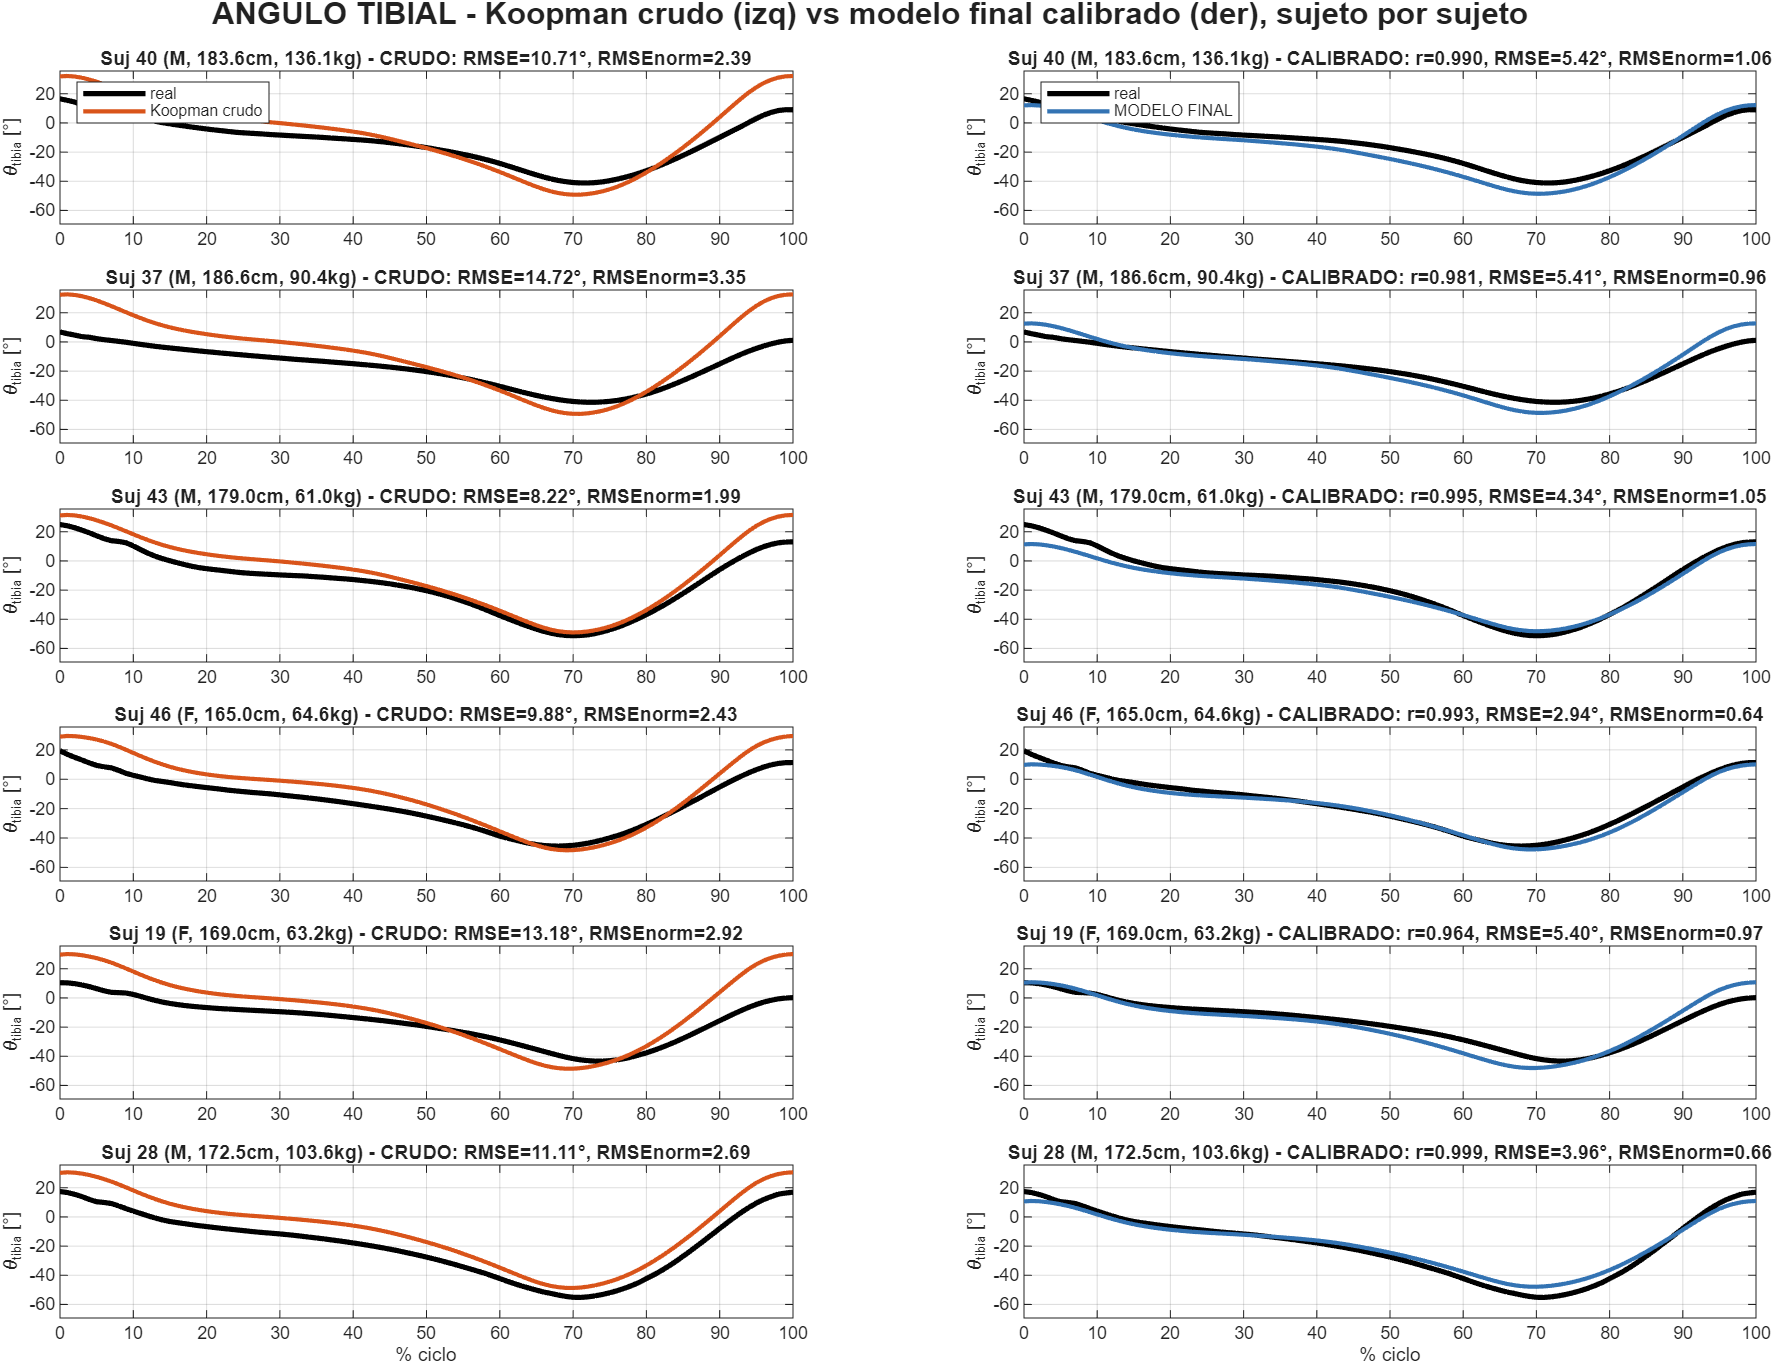
\includegraphics[width=0.8\textwidth]{figuras/11_angulo_tibial_vs_kuopio_individual.png}
\caption{Ángulo tibial, mismos 6 sujetos, sin calibrar vs.\ calibrado, misma escala.}
\label{fig:tibial_individual}
\end{figure}

\subsubsection{Resultado final: comparación completa contra \emph{Kuopio}}
\label{sec:resultados_finales}

\texttt{Correccion\_Hibrida\_PenduloDoble\_Core.m} implementa la corrección de producción: \textbf{Paso 3} (ángulo crudo) $\to$ \texttt{Calibracion\_Koopman\_Kuopio\_Core.m} $\to$ \textbf{Paso 4} (péndulo doble) $\to$ \texttt{Correccion\_Hibrida\_PenduloDoble\_Core.m} (warp en $X$, Ec.~\ref{eq:warp_afin}; Fourier en $Y$, Ec.~\ref{eq:fourier_correccion}). Integrado en \texttt{App\_Animacion\_Cadera\_Rodilla\_Tobillo.m} como DOS interruptores independientes (``Calibrar ángulo (LOSO)'' y ``Corregir posición'', ambos apagados por defecto) --- activar posición fuerza también el ángulo (la corrección de posición se ajustó asumiendo ángulo ya calibrado), pero el ángulo solo sí se puede activar sin la posición.

\begin{table}[H]
\centering
\caption{Resultado final, SOLO TALLA como entrada (LOSO real, $N$=44 para rodilla/tobillo, $N$=47 para ángulo tibial --- mismo pipeline que la app). $X$: warp temporal + afín CONSTANTE (garantiza monotonía en talla), $K_w$=2. $Y$: Fourier, $K$=14. Escala RMSEnorm del proyecto: $<$1 Excelente, $<$1.5 Bueno, $<$2 Aceptable, $>$2 Deficiente (Sección~\ref{sec:metricas}).}
\label{tab:resultados_finales}
\small
\begin{tabular}{@{}llrrl@{}}
\toprule
Segmento & Eje & $r$ & RMSEnorm & Clasificación \\
\midrule
Rodilla ($N=44$) & X & \textbf{0.999} & 1.10 & Bueno \\
Rodilla ($N=44$) & Y & 0.949 & \textbf{0.89} & Excelente \\
Tobillo ($N=44$) & X & \textbf{0.999} & 1.17 & Bueno \\
Tobillo ($N=44$) & Y & \textbf{0.988} & \textbf{0.92} & Excelente \\
\midrule
Ángulo tibial, calibrado ($N=47$) & --- & 0.989 & 1.01 & Bueno \\
\bottomrule
\end{tabular}
\end{table}

\textbf{Las 5 curvas quedan en Excelente o Bueno} --- partiendo de un crudo que, con esta misma métrica, estaba en Deficiente en la mayoría. Las curvas de posición son además continuas, sin escalones ni saltos de velocidad, sin retrocesos, y \textbf{monótonas en talla garantizado} para $X$ (a mayor talla, igual o mayor avance, siempre --- Sección~\ref{sec:retrocesos_x}).

\begin{figure}[H]
\centering
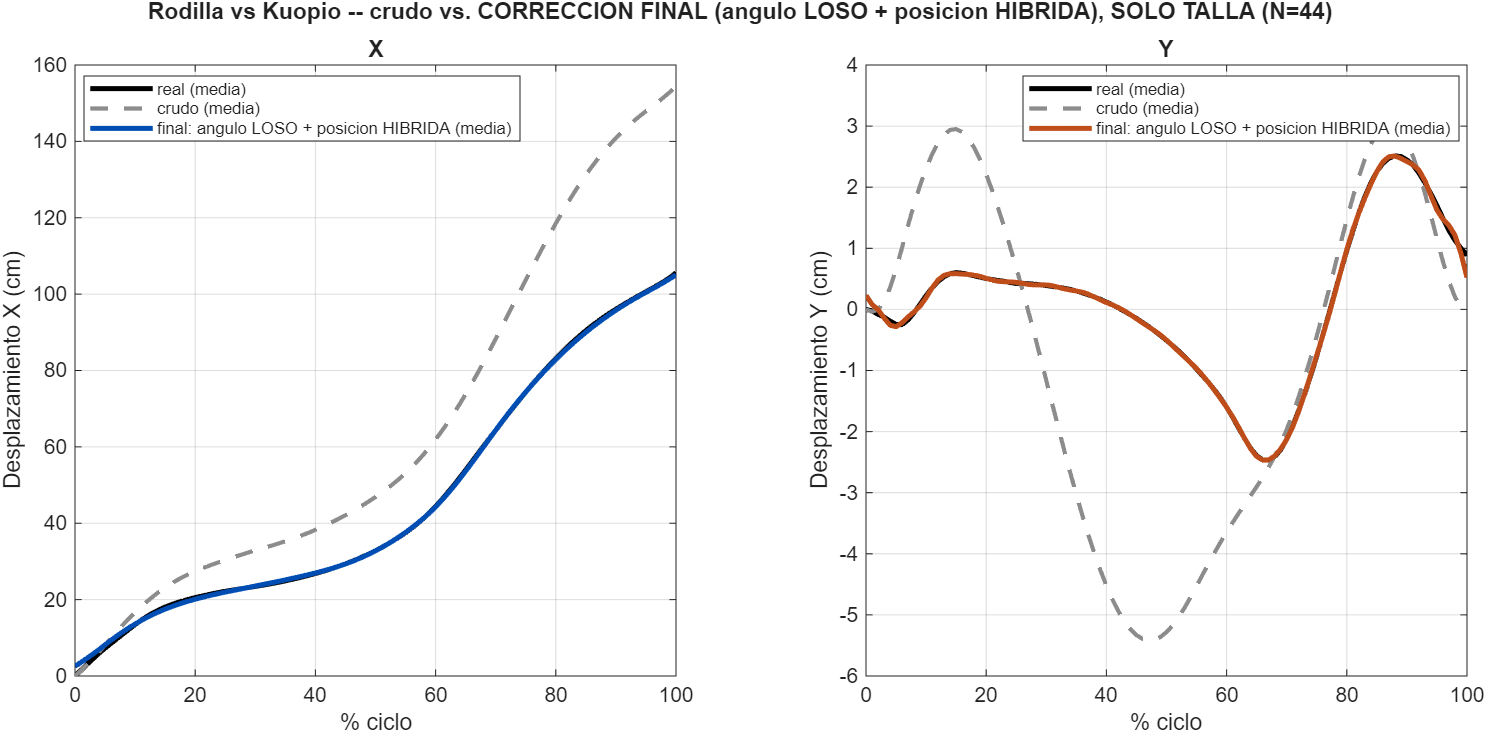
\includegraphics[width=0.8\textwidth]{figuras/06_rodilla_vs_kuopio_grupo.png}
\caption{Desplazamiento final de rodilla: crudo (gris) vs.\ corrección final --- ángulo LOSO + posición híbrida (color) --- vs.\ real (negro) --- 44 sujetos de \emph{Kuopio}, curvas media, SOLO TALLA como entrada.}
\label{fig:rodilla_grupo}
\end{figure}

\begin{figure}[H]
\centering
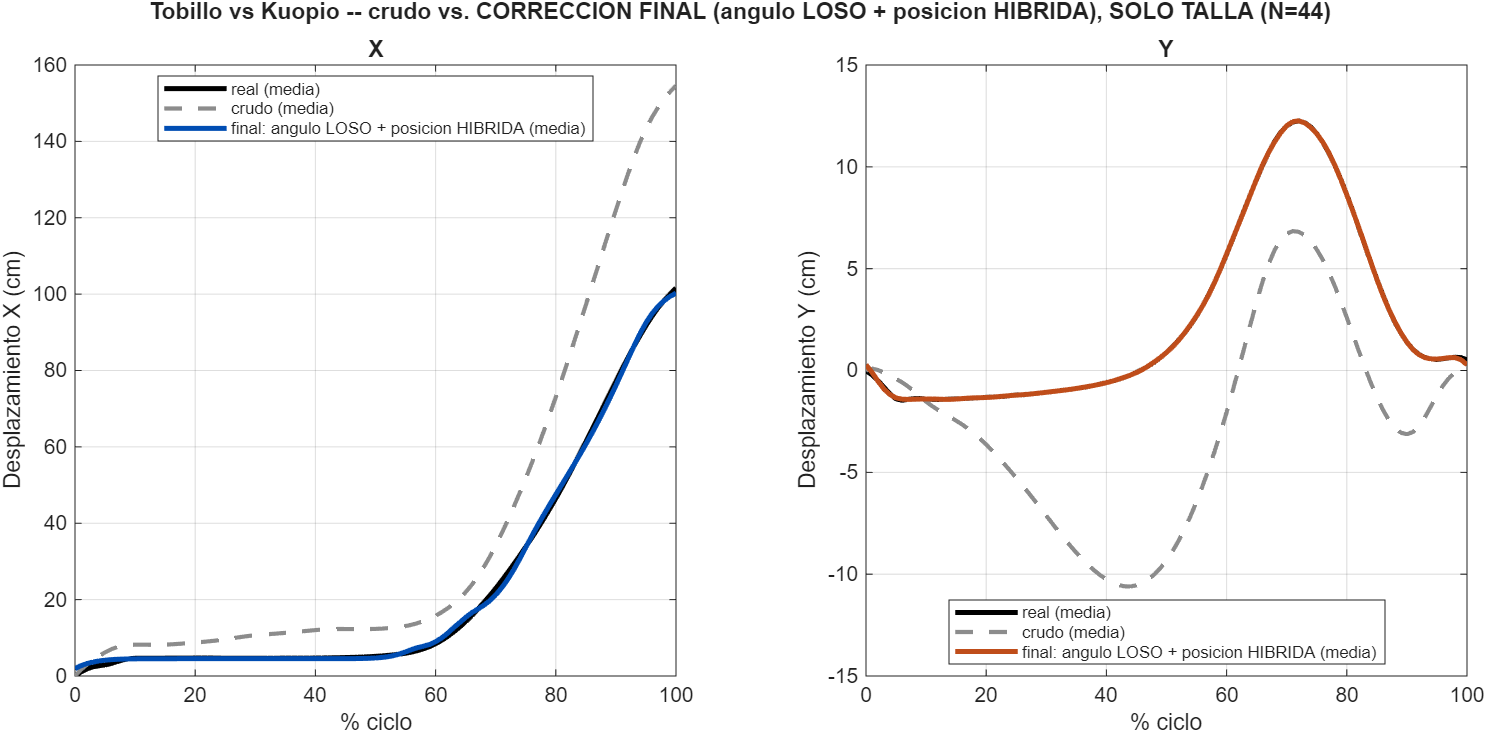
\includegraphics[width=0.8\textwidth]{figuras/08_tobillo_vs_kuopio_grupo.png}
\caption{Desplazamiento final de tobillo, mismo formato que la Figura~\ref{fig:rodilla_grupo}.}
\label{fig:tobillo_grupo}
\end{figure}

\begin{figure}[H]
\centering
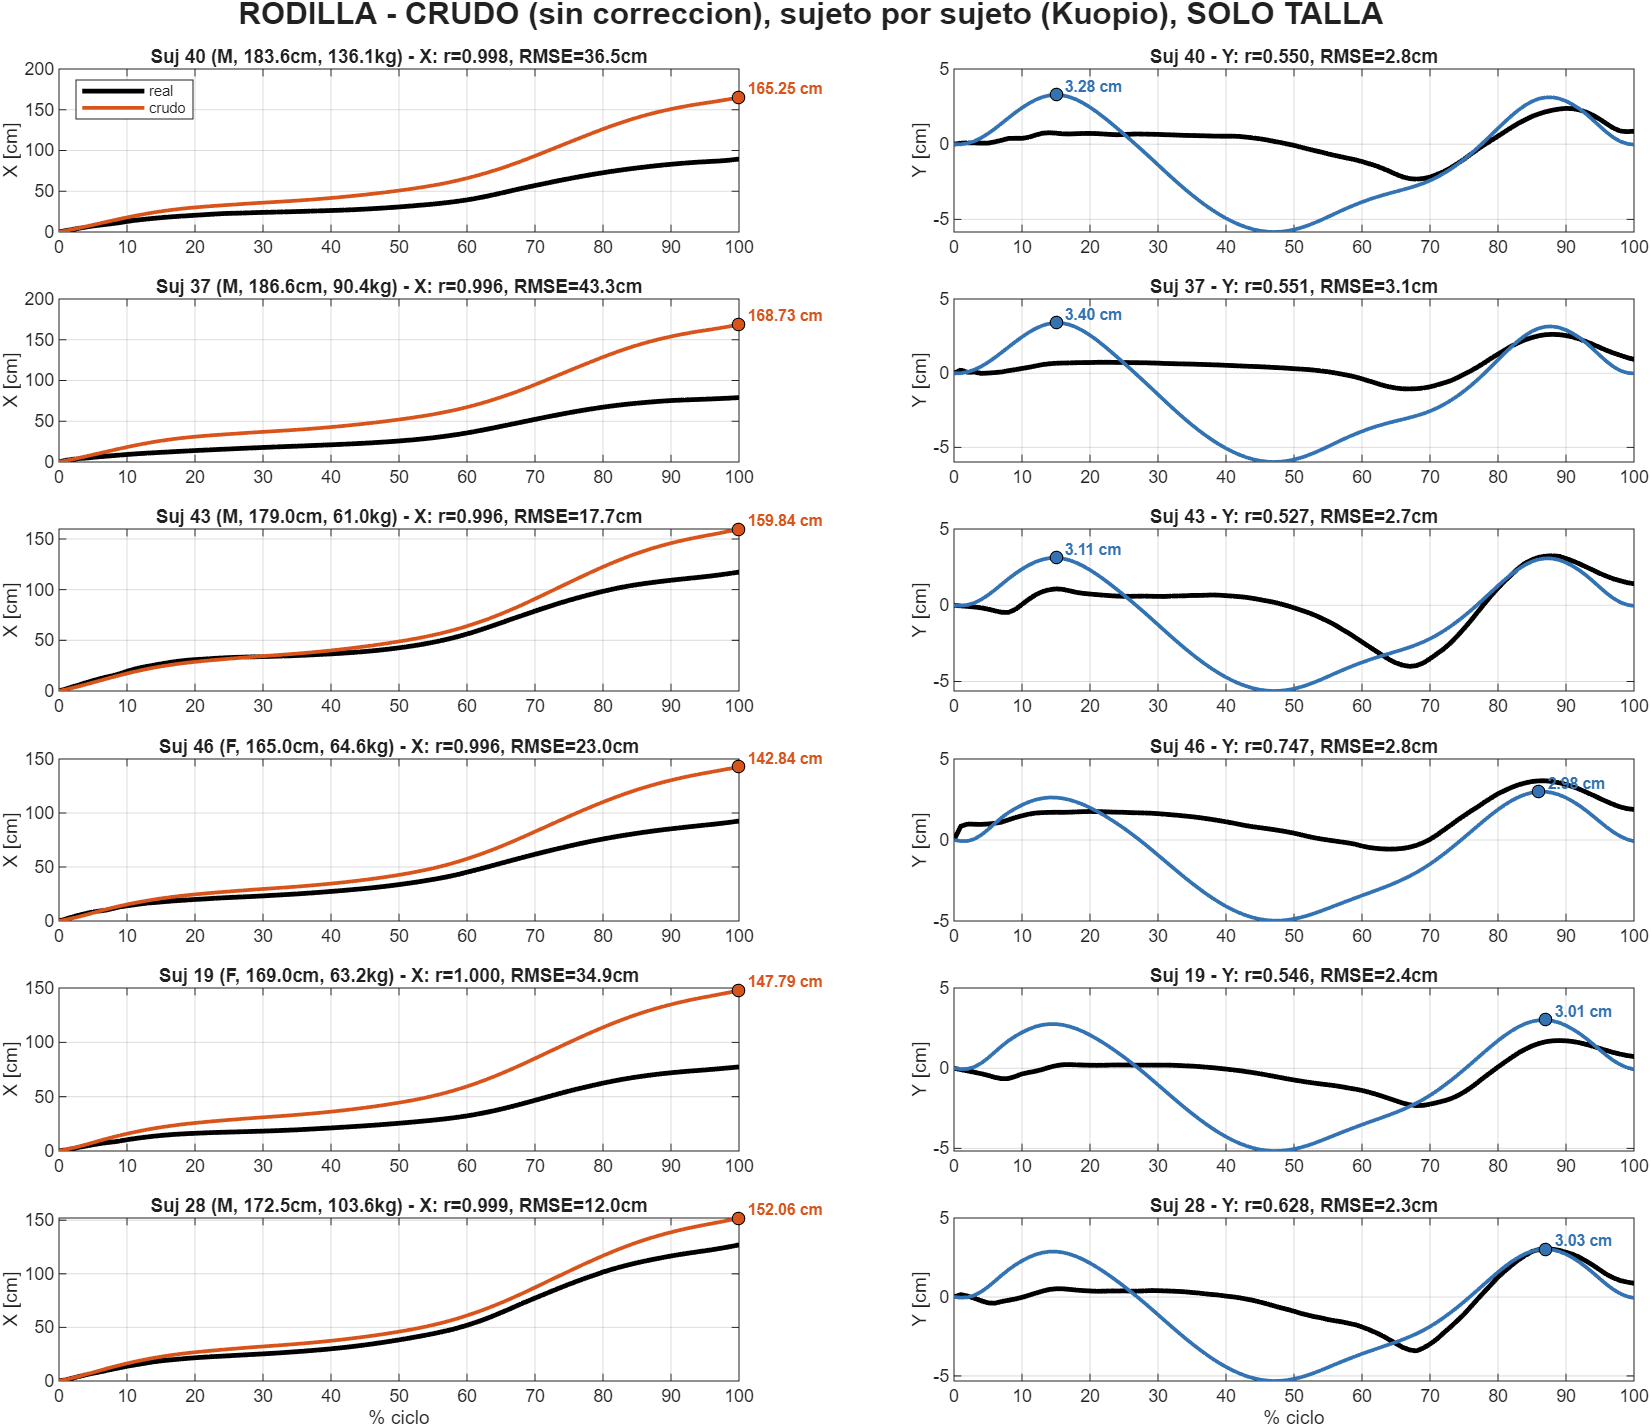
\includegraphics[width=0.8\textwidth]{figuras/07_rodilla_individual_penduloDoble.png}
\caption{Desplazamiento final de rodilla, CRUDO (sin corrección), los 6 sujetos de antropometría más diversa (más pesado, más alto, más liviano, más baja, mujer y hombre de talla media --- mismos 6 sujetos que el resto del proyecto).}
\label{fig:rodilla_individual_pendulo}
\end{figure}

\begin{figure}[H]
\centering
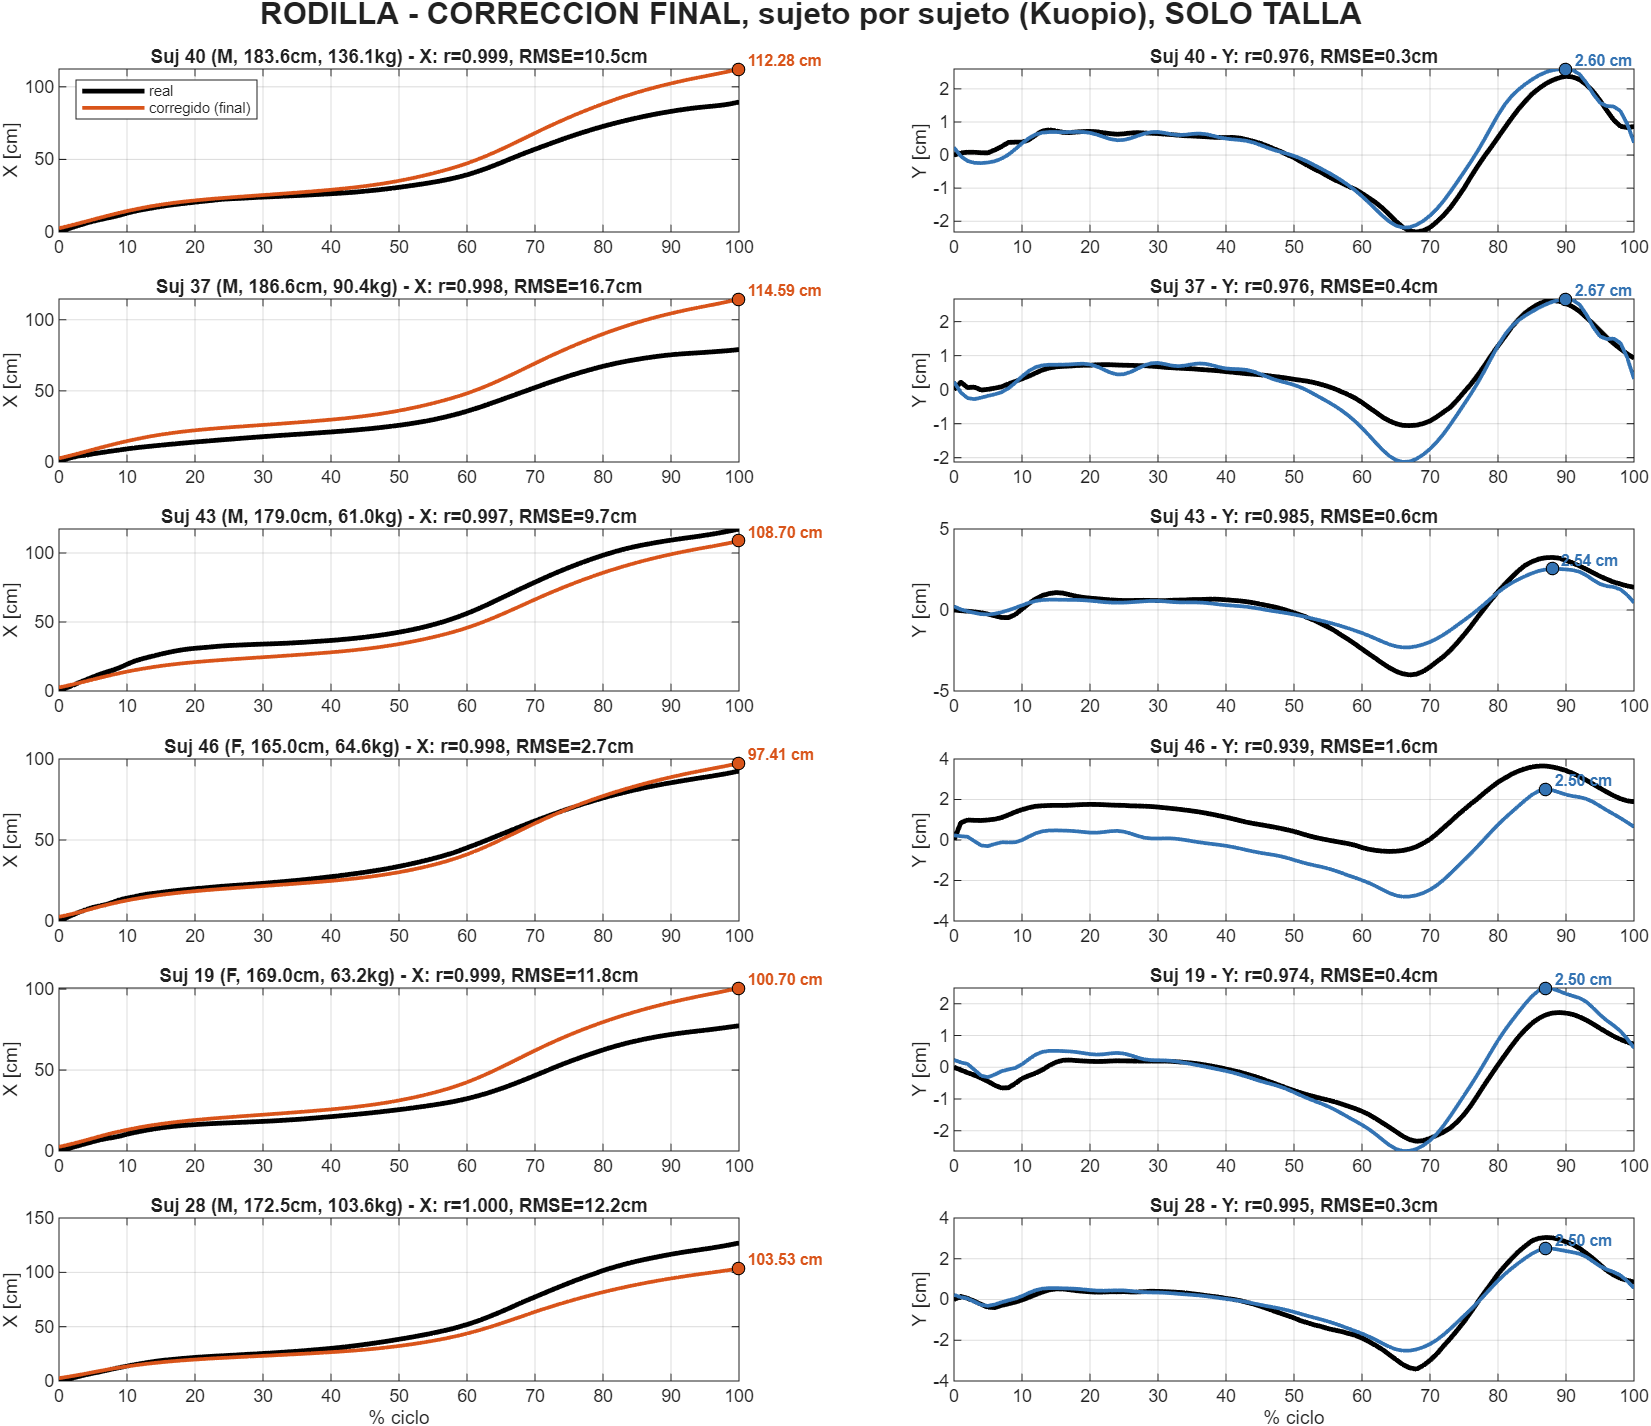
\includegraphics[width=0.8\textwidth]{figuras/07b_rodilla_individual_penduloDoble_calibrado.png}
\caption{Mismo formato que la Figura~\ref{fig:rodilla_individual_pendulo}, CON la corrección final (ángulo LOSO + posición híbrida). El punto y valor marcados son el máximo de la curva predicha --- mismo número que debe mostrar la app con esa talla y la corrección activa.}
\label{fig:rodilla_individual_pendulo_cal}
\end{figure}

\begin{figure}[H]
\centering
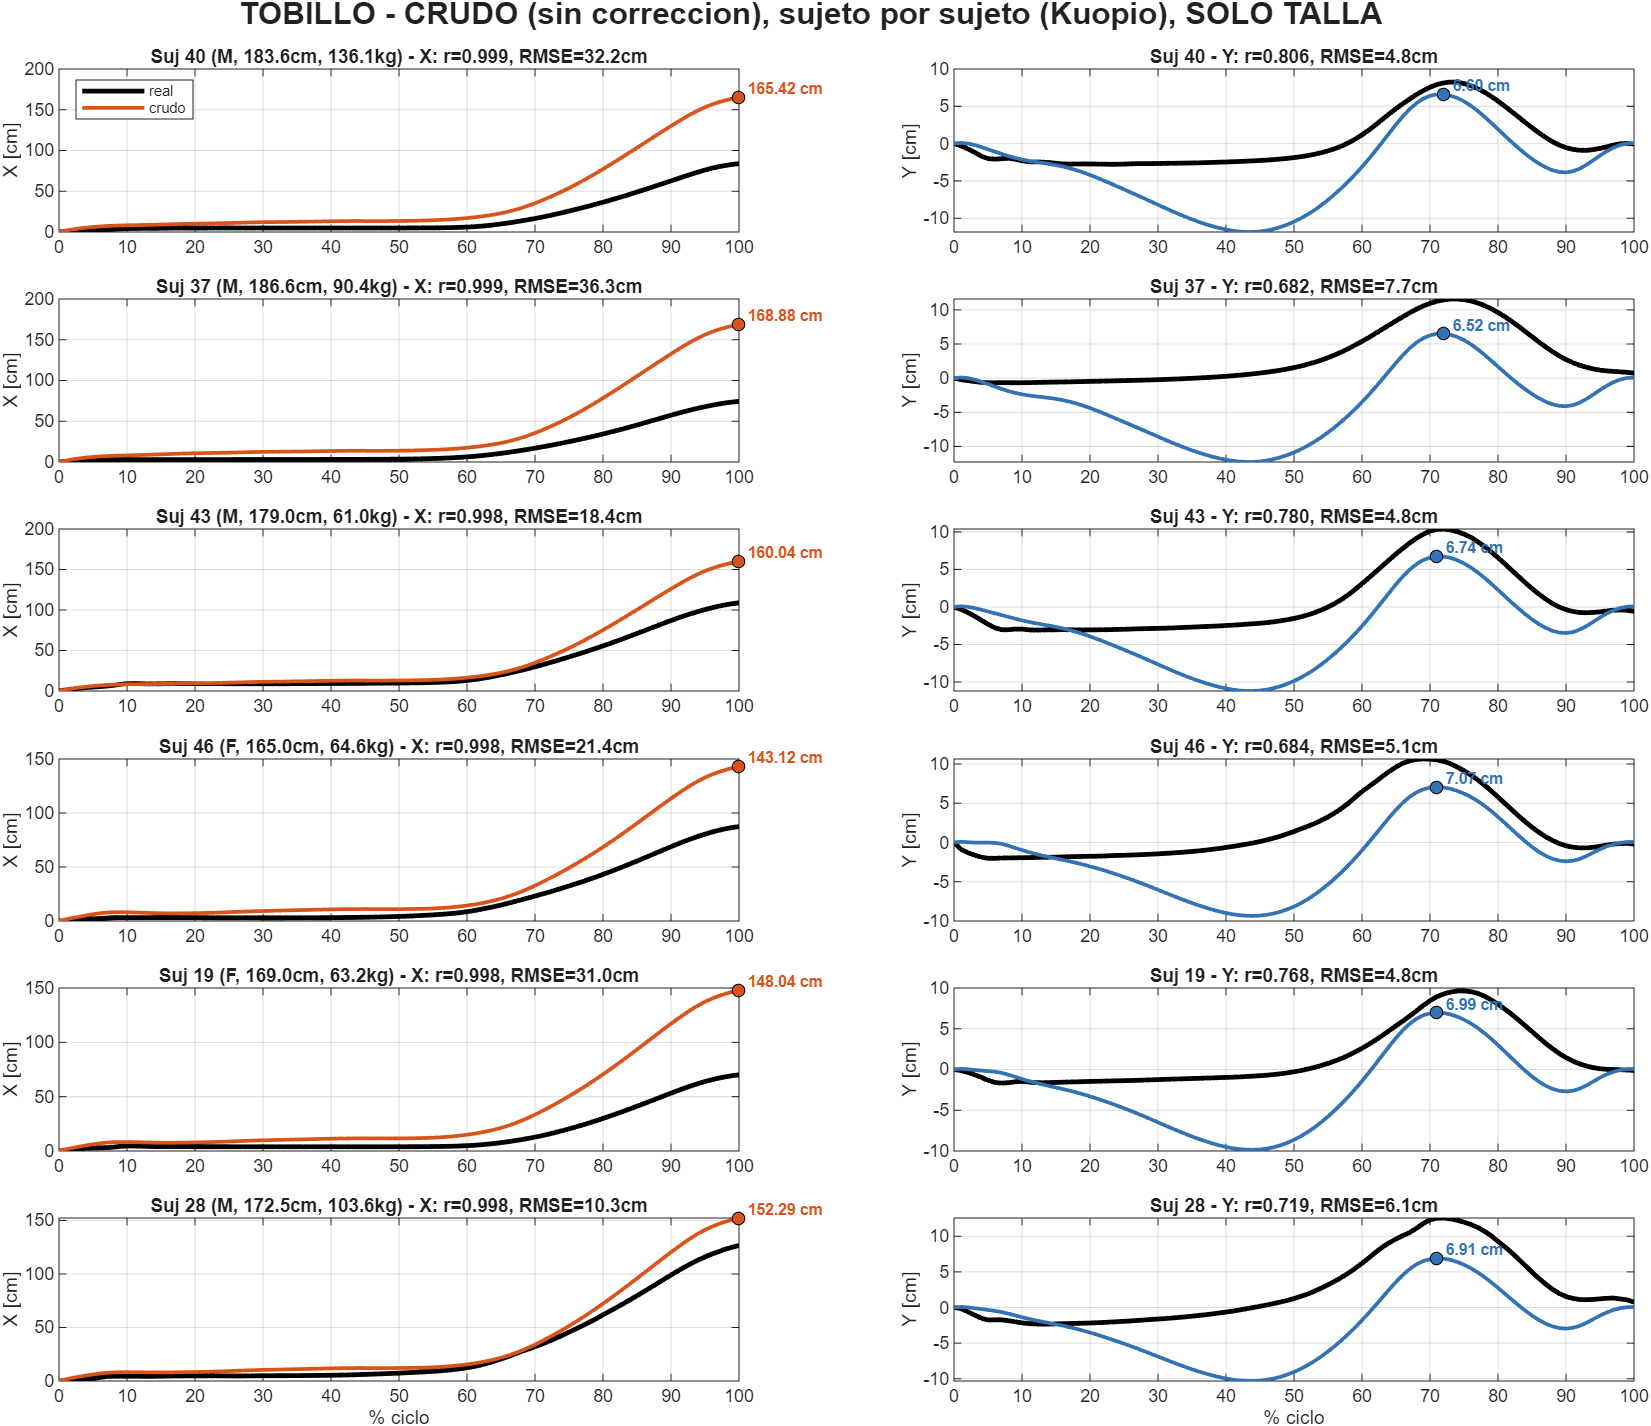
\includegraphics[width=0.8\textwidth]{figuras/09_tobillo_individual_penduloDoble.png}
\caption{Desplazamiento final de tobillo, CRUDO (sin corrección), mismos 6 sujetos de referencia.}
\label{fig:tobillo_individual_pendulo}
\end{figure}

\begin{figure}[H]
\centering
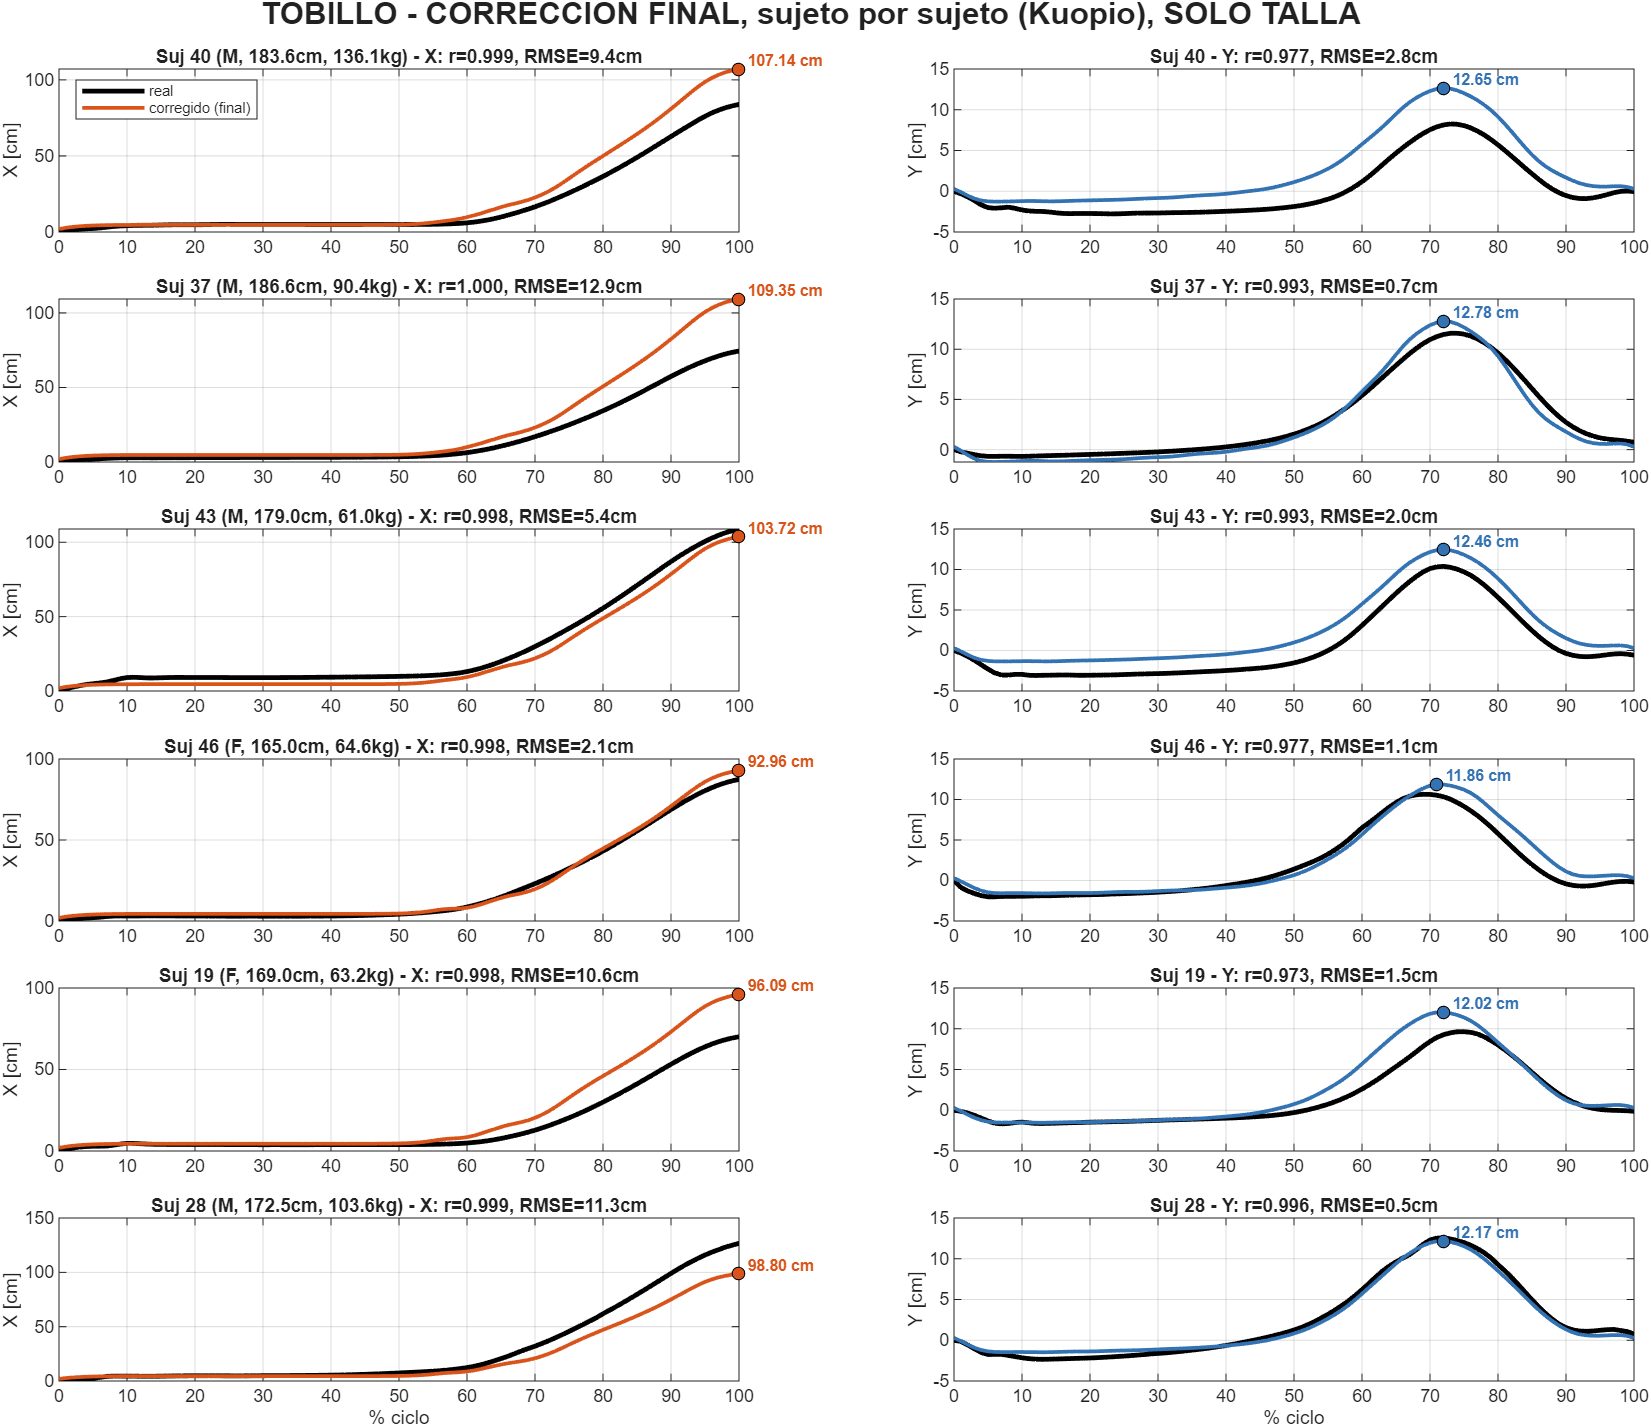
\includegraphics[width=0.8\textwidth]{figuras/09b_tobillo_individual_penduloDoble_calibrado.png}
\caption{Mismo formato que la Figura~\ref{fig:tobillo_individual_pendulo}, CON la corrección final --- la giba de despegue (60--90\,\%) pasa a coincidir muy bien en los 6 sujetos, sin escalones. El punto y valor marcados son el máximo de la curva predicha --- mismo número que debe mostrar la app con esa talla y la corrección activa.}
\label{fig:tobillo_individual_pendulo_cal}
\end{figure}

\paragraph{Desglose: qué aporta cada corrección por separado.} Las figuras anteriores solo muestran crudo total vs.\ resultado final --- se agregan las curvas intermedias (SOLO ángulo LOSO, SIN corrección de posición) para ver qué aporta cada paso, media de los 44 sujetos:

\begin{figure}[H]
\centering
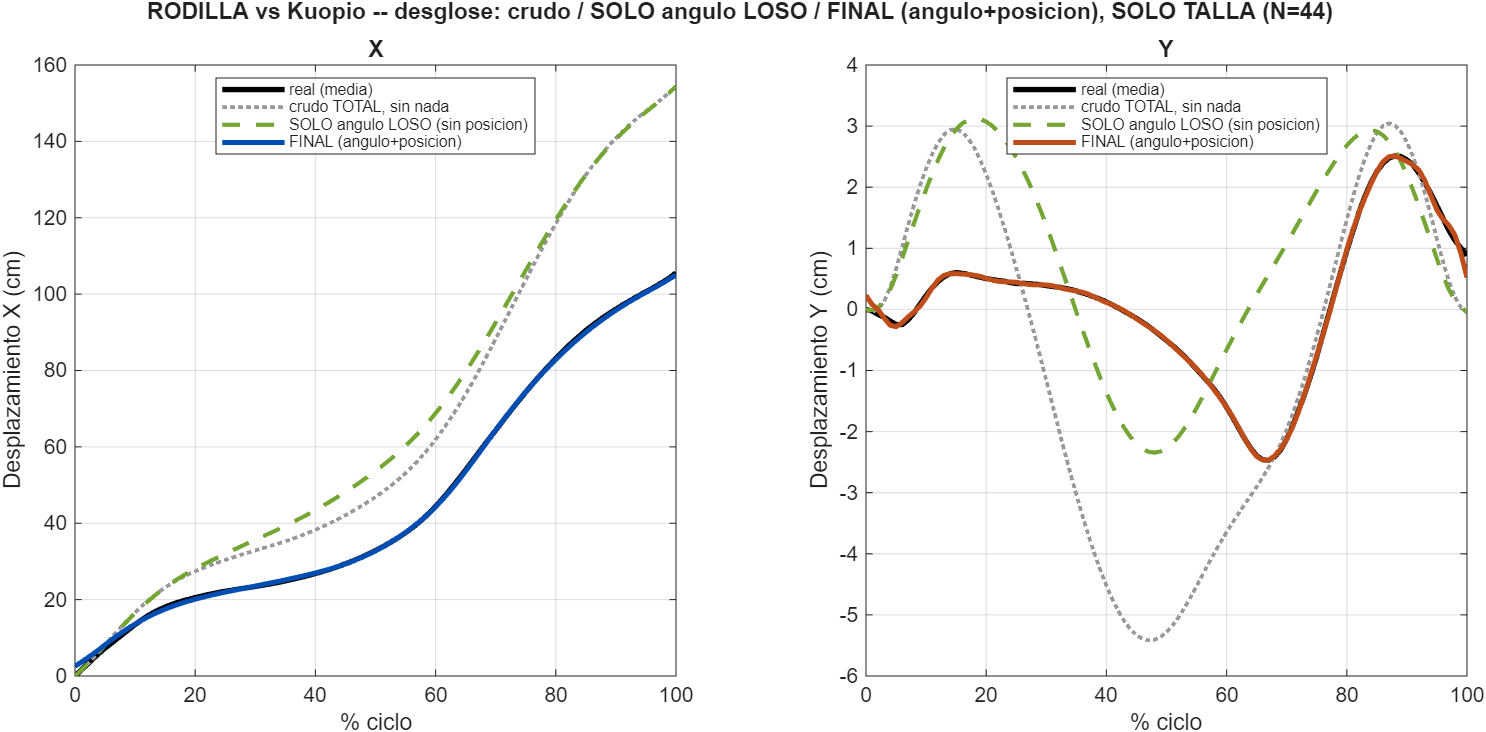
\includegraphics[width=0.95\textwidth]{figuras/12_rodilla_desglose_vs_kuopio_grupo.png}
\caption{Rodilla: desglose de las 2 correcciones. Crudo total (gris punteado) $\to$ SOLO ángulo LOSO, sin corregir posición (verde discontinuo) $\to$ FINAL, ángulo+posición híbrida (color sólido) $\to$ real (negro). En $X$, el ángulo LOSO por sí solo casi no cambia la curva --- es la corrección de \emph{posición} la que hace casi todo el trabajo. En $Y$ es al revés: el ángulo LOSO ya baja el sobrepico de $\sim$5.5\,cm a $\sim$3\,cm, y la corrección de posición cierra el resto hasta $\sim$2.5\,cm (real).}
\label{fig:rodilla_desglose}
\end{figure}

\begin{figure}[H]
\centering
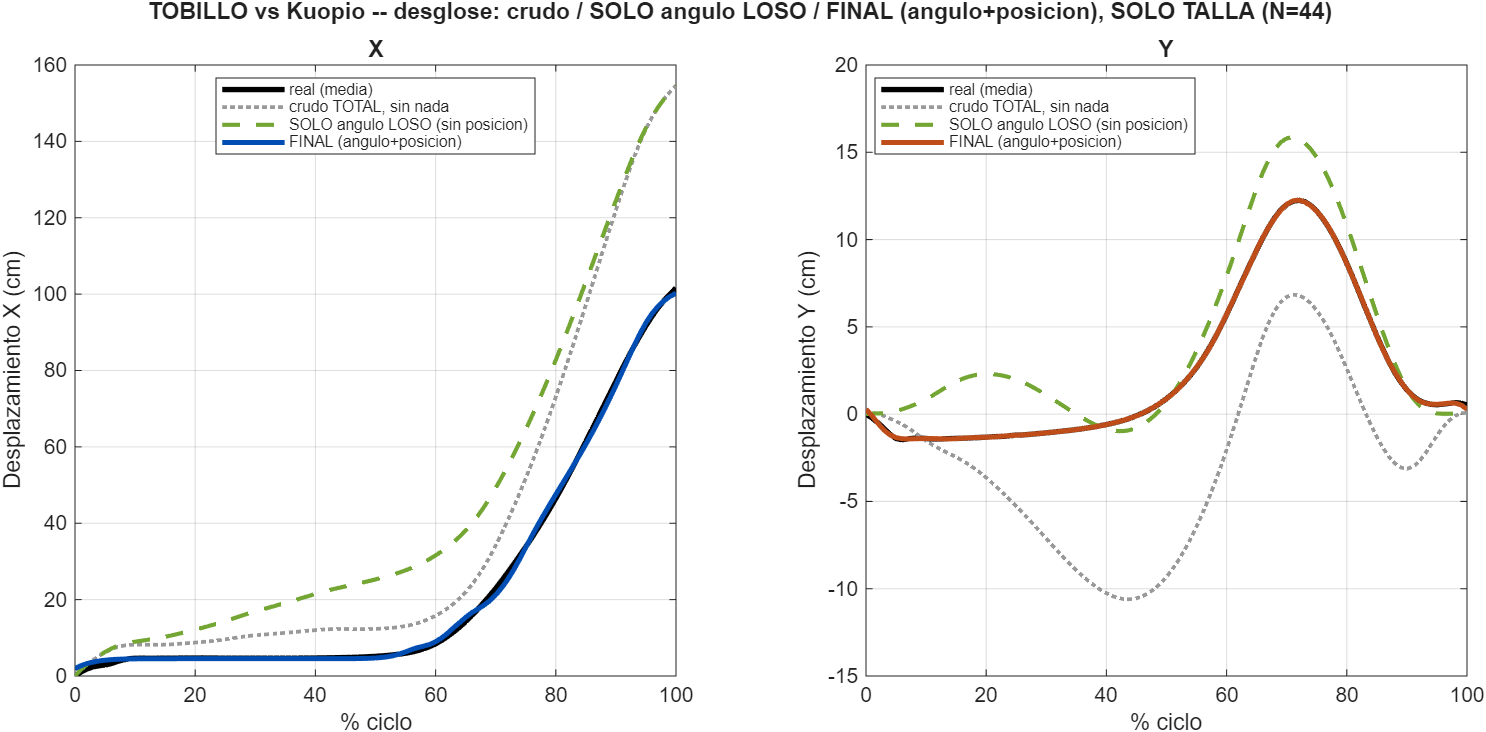
\includegraphics[width=0.95\textwidth]{figuras/13_tobillo_desglose_vs_kuopio_grupo.png}
\caption{Tobillo, mismo formato que la Figura~\ref{fig:rodilla_desglose}.}
\label{fig:tobillo_desglose}
\end{figure}

\subsection{Validación sujeto por sujeto, no con curvas promedio}
\label{sec:validacion_individual}

\aporte{Promediar curvas de cuerpos distintos mezclaría trayectorias no comparables --- por eso las Figuras~\ref{fig:rodilla_grupo}--\ref{fig:tobillo_grupo} ya muestran las 44 curvas individuales, no solo un promedio.} Se conserva además, para los tres segmentos (rodilla, tobillo, ángulo tibial), la validación contra los MISMOS 6 sujetos de antropometría deliberadamente diversa (más pesado, más alto, más liviano, más baja, mujer y hombre de talla media --- sujetos 40/37/43/46/19/28) --- Figuras~\ref{fig:rodilla_individual_pendulo}--\ref{fig:rodilla_individual_pendulo_cal} (rodilla), \ref{fig:tobillo_individual_pendulo}--\ref{fig:tobillo_individual_pendulo_cal} (tobillo) y \ref{fig:tibial_individual} (ángulo tibial), ninguno con falla notoria. Los 6 sujetos son deliberadamente los mismos en los tres segmentos, para poder comparar el desempeño del modelo sujeto a sujeto.

\section{Por qué Koopman: búsqueda y comparación de candidatos}
\label{sec:busqueda}

\textbf{Esta sección se lee al final a propósito, no por descuido:} todo lo anterior (Secciones~\ref{sec:koopman}--\ref{sec:resultados}) ya mostró el flujo completo de un solo modelo --- Koopman, calibrado, validado. Lo que sigue aquí es la evidencia de \emph{por qué} se eligió Koopman sobre los otros dos candidatos serios (Zhao, Yun) --- respaldo de la decisión, no un requisito para entender lo ya leído.

Criterio de inclusión, fijado \emph{antes} de ver resultados:
\begin{enumerate}
    \item coeficientes ya ajustados y publicados, reutilizables sin reentrenar;
    \item entrada = antropometría estática (talla, masa, sexo) + a lo sumo velocidad de marcha, nunca un sensor en tiempo real.
\end{enumerate}

12 candidatos investigados a fondo (4 con el artículo completo leído línea por línea). Figura~\ref{fig:flujo_seleccion}.

\begin{figure}[H]
\centering
\begin{tikzpicture}[
  node distance=0.9cm and 1.2cm,
  box/.style={draw, rectangle, rounded corners, align=center, minimum width=7.4cm, minimum height=1.05cm, font=\small},
  smallbox/.style={draw, rectangle, rounded corners, align=center, minimum width=4.9cm, minimum height=1.3cm, font=\small},
  >=Stealth
]
\node[box] (n1) {12 candidatos identificados\\(modelos publicados de predicción de cinemática de marcha)};
\node[box, below=of n1] (n2) {Criterio de inclusión: coeficientes ya publicados y reutilizables sin\\reentrenar + entrada de antropometría estática (más velocidad, medida o estimada)};
\node[smallbox, below left=1.1cm and 0.3cm of n2] (n3) {8 descartados\\(Tabla~\ref{tab:descartados})};
\node[smallbox, below right=1.1cm and 0.3cm of n2] (n4) {4 candidatos viables};
\node[smallbox, below left=1.3cm and -0.2cm of n4] (n5) {3 evaluados a fondo en\\rodilla, tobillo e inclinación tibial:\\Koopman 2014, Zhao 2026, Yun 2014};
\node[smallbox, below right=1.3cm and -0.2cm of n4] (n6) {1 excluido de la comparación final:\\Romero-Sorozábal et al.\ 2024\\(anomalía de escala en eje vertical)};

\draw[->] (n1) -- (n2);
\draw[->] (n2) -- (n3);
\draw[->] (n2) -- (n4);
\draw[->] (n4) -- (n5);
\draw[->] (n4) -- (n6);
\end{tikzpicture}
\caption{Proceso de selección de modelos candidatos, de 12 identificados a 3 evaluados en los tres segmentos de interés de este informe.}
\label{fig:flujo_seleccion}
\end{figure}

\begin{table}[H]
\centering
\caption{Los 8 candidatos descartados y el motivo verificado de exclusión.}
\label{tab:descartados}
\small
\begin{tabular}{@{}p{3.0cm}p{2.6cm}p{7.6cm}@{}}
\toprule
Candidato & Método & Motivo de exclusión \\
\midrule
Hu et al.\ 2020 & Regresión LASSO & No publica los coeficientes del modelo (verificado a texto completo) \\
Luu et al.\ 2014 & GRNN & Requiere la base de entrenamiento completa (600 caminatas, 70 sujetos), no solo coeficientes \\
Wu et al.\ 2018 & Autoencoder + GPR & Matrices de pesos no publicadas; además no predice tobillo \\
Luu et al.\ 2011 & Red neuronal (MLPNN) & Pesos entrenados no publicados \\
Semwal et al.\ 2023 & LSTM + CNN & Modelo de caja negra, sin pesos publicados \\
Xin et al.\ 2025 & GPR + coeficientes de Fourier & Sin verificación posible a la fecha de esta búsqueda \\
Shkedy Rabani et al.\ 2022 & Modelo biomecánico & No personaliza por antropometría, solo por pendiente del terreno \\
Al Kouzbary et al.\ 2026 & Modelo híbrido & Requiere ángulo tibial medido en tiempo real como entrada \\
\bottomrule
\end{tabular}
\end{table}

De los 4 candidatos viables, 3 (Koopman~\cite{Koopman2014}, Zhao~\cite{Zhao2026}, Yun~\cite{Yun2014}) entregan ángulos articulares clásicos y se evaluaron a fondo (Sección~\ref{sec:resultados}). El cuarto, Romero-Sorozábal et al.\ (2024), da posición 3D directa pero su eje vertical de rodilla/tobillo tiene una anomalía de escala verificada dos veces en la propia fuente --- excluido de la comparación final, fuera del alcance de este informe.

\aporte{De los 12 candidatos, solo 33\,\% publica parámetros reutilizables sin reentrenar --- problema de reproducibilidad del campo, no de esta búsqueda.}

\subsection{Comparación entre los tres candidatos}
\label{sec:comparacion_candidatos}

Tabla~\ref{tab:comparacion_rodilla}: correlación ($r$) de los 3 candidatos vs.\ posición/ángulo de rodilla medido, por fuente.

\begin{table}[H]
\centering
\caption{Correlación ($r$) de los tres candidatos frente a la posición o ángulo de rodilla medido, por fuente de datos.}
\label{tab:comparacion_rodilla}
\small
\begin{tabular}{@{}lrrrr@{}}
\toprule
Fuente & $n$ & Koopman & Zhao & Yun \\
\midrule
Registro propio & 1 & 0.982 & $-$0.21 & $-$0.28 \\
Winter~\cite{Winter2009} & 1 & 0.816 & 0.613 & 0.468 \\
Maastricht~\cite{Senden2024} & 246 & 0.933 & 0.982\textsuperscript{a} & 0.955\textsuperscript{a} \\
Ferber ($r_x$)~\cite{Ferber2024} & 40 & 0.945 & 0.947\textsuperscript{b} & 0.902 \\
Ferber ($r_y$)~\cite{Ferber2024} & 40 & 0.791 & 0.815\textsuperscript{b} & $-$0.698 \\
Kuopio, calibrado ($r_x$/$r_y$)~\cite{Lavikainen2024} & 15 & 0.998 / 0.920 & no eval. & no eval. \\
\bottomrule
\end{tabular}

\vspace{0.15cm}
\footnotesize\textsuperscript{a}~lado desplazado en fase (ver texto). \quad \textsuperscript{b}~lado nativo, sin ajuste.
\end{table}

\aporte{Hallazgo propio: el resultado de Zhao/Yun arriba parece contradictorio a primera vista (negativo en registro propio/Winter, positivo en Maastricht, mismo "lado"). Verificado numéricamente: el parámetro de "lado" de Zhao no es un espejo anatómico, sino un desfase de fase de 50\,\% del ciclo aplicado por igual a cadera y rodilla. La rodilla de Zhao tiene un defecto real (pico en 22\,\% del ciclo, no $\sim$70\,\%) que el desfase corrige por coincidencia ($22+50=72\,\%$); pero la cadera de Zhao, sin ese defecto (pico ya en 83\,\%), se rompe con el mismo desfase (queda en 33\,\%). Ferber deriva rodilla de cadera; Maastricht mide rodilla directo --- cada base "premia" un lado distinto del mismo defecto. Confirmado igual en tobillo y ángulo tibial (Tabla~\ref{tab:comparacion_tobillo_tibial}); en ninguna pieza Zhao/Yun superan a Koopman.}

\begin{table}[H]
\centering
\caption{Correlación y RMSE frente a tobillo y ángulo tibial, \emph{Kuopio} ($n=15$), configuración nativa (sin desfase de lado).}
\label{tab:comparacion_tobillo_tibial}
\small
\begin{tabular}{@{}lrrr@{}}
\toprule
& Koopman & Zhao & Yun \\
\midrule
Tobillo X: $r$ / RMSE (cm) & 0.998 / 2.90 & 0.974 / 10.99 & 0.990 / 7.08 \\
Tobillo Y: $r$ / RMSE (cm) & 0.985 / 1.54 & 0.914 / 2.51 & 0.831 / 3.39 \\
Ángulo tibial: $r$ crudo & 0.992 & $-$0.303 & $-$0.300 \\
Ángulo tibial: RMSEnorm calibrado & 0.92 (Excelente) & 3.39 (Deficiente) & 4.42 (Deficiente) \\
\bottomrule
\end{tabular}
\end{table}

Figuras~\ref{fig:seleccion_control}--\ref{fig:cuatro_candidatos}: selección progresiva de Koopman (registro propio $\to$ Maastricht $\to$ Ferber) y cadena cinemática comparada de los 4 candidatos.

\begin{figure}[H]
\centering
\begin{subfigure}[t]{0.32\textwidth}
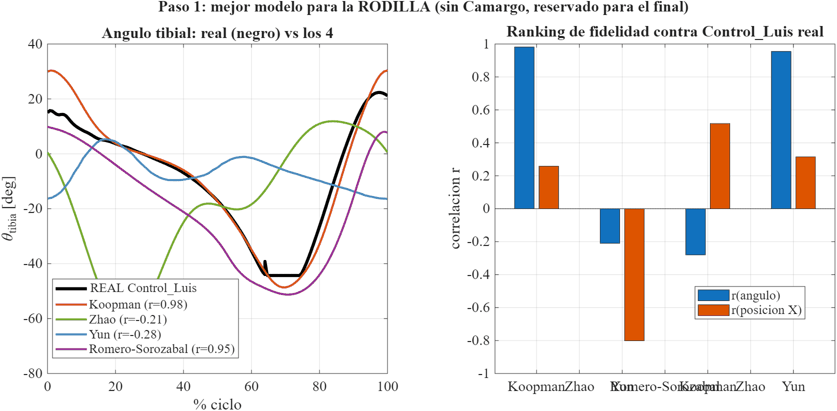
\includegraphics[width=\textwidth]{figuras/01_seleccion_koopman_vs_control_luis.png}
\caption{}
\label{fig:seleccion_control}
\end{subfigure}
\hfill
\begin{subfigure}[t]{0.32\textwidth}
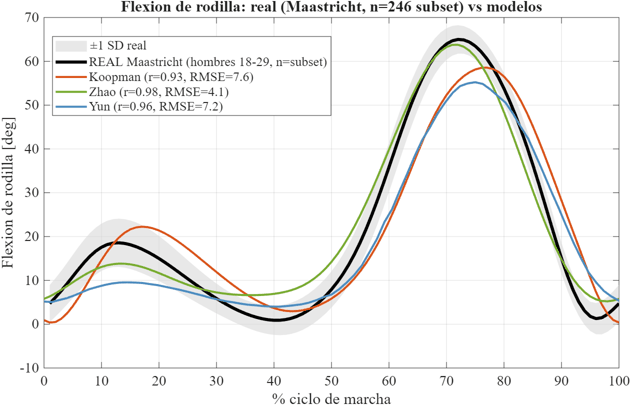
\includegraphics[width=\textwidth]{figuras/02_seleccion_koopman_vs_maastricht.png}
\caption{}
\label{fig:seleccion_maastricht}
\end{subfigure}
\hfill
\begin{subfigure}[t]{0.32\textwidth}
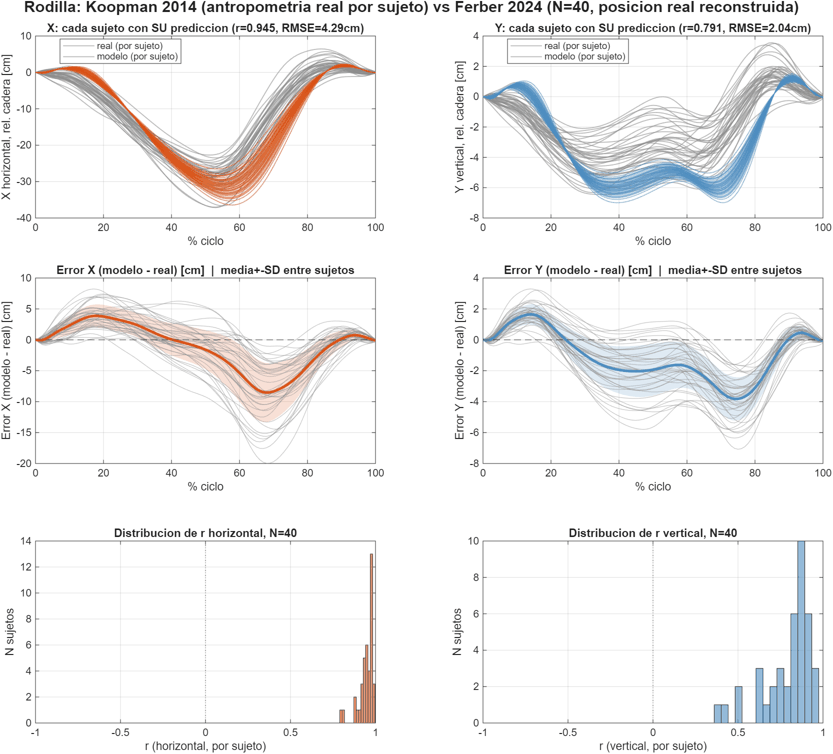
\includegraphics[width=\textwidth]{figuras/03_seleccion_koopman_vs_ferber.png}
\caption{}
\label{fig:seleccion_ferber}
\end{subfigure}
\caption{Selección progresiva de Koopman: (a) registro propio ($n=1$, $r=0.982$); (b) Maastricht ($n=246$); (c) Ferber ($n=40$, posición 3D real).}
\label{fig:seleccion_progresiva}
\end{figure}

\begin{figure}[H]
\centering
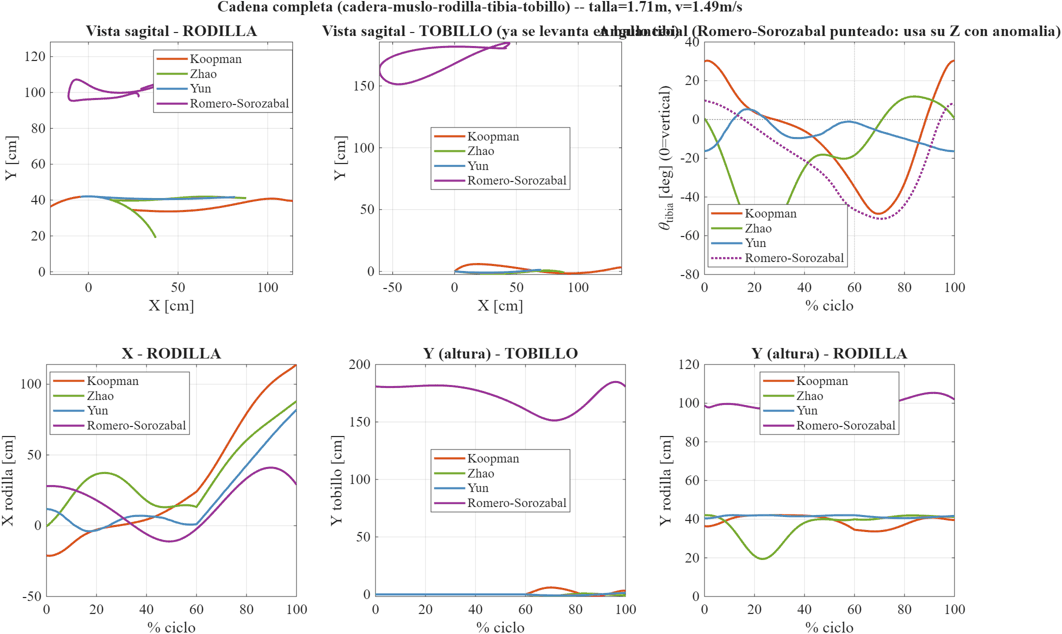
\includegraphics[width=0.85\textwidth]{figuras/04_los_4_candidatos_cadena_completa.png}
\caption{Cadena cinemática completa (cadera-rodilla-tobillo) de los 4 candidatos investigados a fondo, lado a lado --- se observa la flexión de rodilla insuficiente de Zhao y Yun en balanceo, consistente con el defecto de fase.}
\label{fig:cuatro_candidatos}
\end{figure}

\section{Limitaciones}
\label{sec:limitaciones}

\begin{itemize}
    \item \textbf{Los coeficientes de la corrección final (ángulo LOSO + posición híbrida: warp en $X$, Fourier en $Y$) se ajustaron con los 44 sujetos de \emph{Kuopio}} (sanos, sin prótesis, talla 161--186.6\,cm) --- aplicarlos a un usuario protésico o fuera de ese rango de talla/velocidad es extrapolación, misma limitación ya declarada para la calibración de ángulo (Sección~\ref{sec:calibracion}). Probado explícitamente en los extremos permitidos por la app (130 y 210\,cm, 31-ago-2026): no produce valores absurdos, pero el comportamiento fuera del rango validado no tiene respaldo de dato real --- la app muestra una advertencia visible cuando la talla ingresada cae fuera de 161--186.6\,cm.
    \item \textbf{Nota de consistencia interna (encontrada al preparar esta versión):} los coeficientes de la Tabla~\ref{tab:coeficientes_calibracion} (0.769/$-2.69^\circ$; 0.811/$-11.33^\circ$) son el \emph{promedio de los 15 pliegues LOSO}, usados para \emph{validar} --- los números de este informe. La calibración usada para \emph{producción} (28-ago-2026) usa en cambio un ajuste agrupado sobre $N=13$ sujetos (2 de los 15 no tienen el marcador de tibia completo en el archivo crudo), dando 0.7609/$-2.00^\circ$ y 0.8123/$-11.35^\circ$ --- cercano pero no idéntico. No cambia ninguna conclusión (mismo orden de magnitud, misma dirección de corrección), pero conviene que el artículo final declare cuál de los dos conjuntos de coeficientes usa.

    \item Velocidad estimada por Froude (Ec.~\ref{eq:froude}) supera el rango validado por Koopman (0.5--5\,km/h) para la mayoría de tallas adultas --- extrapolación declarada. Camargo sigue siendo el examen final de no-circularidad, no ejecutado todavía.

    \item Signo de la componente vertical del generador (Ec.~\ref{eq:cadera_y}) no se ha contrastado todavía contra el sentido real del eje vertical del CSV que lee el simulador --- pendiente antes de conectar el Paso 4 nuevo al exportador (\texttt{Escribir\_CSV\_Simulador.m} sigue leyendo del enfoque anterior, Sección~\ref{sec:paso5}).

    \item \texttt{Escribir\_CSV\_Simulador.m} y \texttt{Generar\_Trayectoria.m} todavía leen del enfoque de posición ANTERIOR al Paso 4 nuevo --- conectarlos es trabajo pendiente, no hecho en esta sesión.

    \item \textbf{Retrocesos en X: RESUELTO} (Sección~\ref{sec:retrocesos_x}) --- la corrección híbrida (warp temporal + afín constante en X, Fourier sin cambio en Y) elimina los retrocesos por construcción matemática (0/100 en rodilla y tobillo, LOSO $N$=44), no solo empíricamente, y garantiza además que el avance final sea monótono en talla. Limitación que queda: el warp se ajustó con los mismos 44 sujetos de \emph{Kuopio} (talla 161--186.6\,cm) --- misma extrapolación fuera de ese rango ya declarada para el resto de las correcciones.

    \item Comparación completa contra Camargo et al.~\cite{Camargo2021}, examen final de no-circularidad, todavía no ejecutada --- prioridad más alta pendiente.

    \item Zhao~\cite{Zhao2026} y Yun~\cite{Yun2014} tienen el defecto de fase de rodilla (Sección~\ref{sec:comparacion_candidatos}), no corregible sin reajustar coeficientes originales --- quedan como candidatos de comparación, no como modelo principal.

    \item \textbf{Ángulo tibial: la variabilidad entre sujetos que predice el modelo es mucho menor que la real, y en el punto de mayor variabilidad real (${\sim}$70\,\% del ciclo) tiene el signo cambiado respecto a talla.} Verificado numéricamente (01-sep-2026): a 70\,\% del ciclo, SD entre sujetos real = 8.78\textdegree\ vs.\ SD predicha (crudo o calibrado) = 0.33--0.35\textdegree\ (${\sim}$25 veces menor); $corr(talla, real)=+0.27$ (débil) vs.\ $corr(talla, crudo)=-0.97$ (fuerte, signo opuesto). Causa mecánica identificada: $corr(v_{froude}, crudo)=-0.996$ en ese punto, y la velocidad Froude-estimada para estos sujetos (5.21--5.61\,km/h) cae fuera del rango que Koopman 2014 validó (0.5--5\,km/h) --- la extrapolación, aunque pequeña, produce una sensibilidad a velocidad artificialmente fuerte justo ahí. Mismo mecanismo general que la extrapolación de Froude ya declarada arriba, pero aquí cuantificado y con el efecto de signo invertido, no solo de magnitud. Sin corregir en esta versión --- candidato a revisar antes del artículo final (¿acotar/suavizar la sensibilidad a velocidad de Koopman en ese tramo del ciclo?).

    \item Este informe valida cinemática predicha vs.\ medida en bases públicas; no valida que el simulador físico ejecute esa trayectoria con fidelidad (de CSV a posición real de motores) --- pendiente de la integración Raspberry Pi--ESP32 y de la calibración del cero físico del banco (equipo de mecatrónica).
\end{itemize}

\bibliographystyle{unsrt}
\bibliography{referencias_informe}

\end{document}
